\chapter{Evaluation and Results} \label{chap:evaluation}
Unfortunately, there are no publicly available benchmarks for 360\degree image synthesis with 2-DoF without 3D geometry, as not many methods exist that try to achieve this. Since the approach presented in Chapter~\ref{chap:implementation} is a first attempt at solving this problem, this chapter presents a basic evaluation of the algorithm, relying on mathematically calculable error metrics. These metrics measure the accuracy of a synthesized image compared to the ground truth and are used to assess the effect of a limited number of parameters. Using these metrics, it is possible to measure the performance of the 2-DoF synthesis using regular blending, and the 2-DoF synthesis using flow-based blending and compare the two.
%Furthermore, it compares the results of regular blending, flow-based blending, and a na\"ive baseline algorithm to analyze whether, and in which cases an improvement could be achieved.
``Performance'' in the context of this evaluation is defined as the accuracy of the synthesized image based on the error metrics, as well as visual examination.

In order to understand the evaluation process,
 possible parameters of the algorithm and of the scene are discussed (Section~\ref{sec:params}), followed by the presentation of the evaluation methodology (Section~\ref{sec:eval_methodology}).
Then, virtually generated scenes are used to evaluate the effect of different combinations of select parameters in a controlled environment (Section~\ref{sec:limit_eval}).
Based on the knowledge gained in the evaluation on virtual scenes, a proof-of-concept evaluation is performed on a real scene (Section~\ref{sec:pof_eval}). Finally, the limitations of the evaluation are discussed (Section~\ref{sec:limitations}).


%First the evaluation methodology is presented, outlining how the effects of a parameter are measured and evaluated. Then, the limits of the algorithm are explored using virtual scenes. With the information gleaned from this limit evaluation, the parameters are chosen for a proof-of-concept evaluation using real scenes. The results and limitations are then discussed\ldots

%- what is a scenario what is a scene
%- not performance
%- konkreter
%- wie gut koennen szenen synthetisiert werden
%- scope: basic evaluation of mathematically measurable values (no human perception)
%- these datasets could be used in the future to compare different algorithms

\section{Parameters} \label{sec:params}
Before defining the parameters to test in the limitation and proof-of-concept evaluations, this section gives an overview of possible parameters in the context of the 2-DoF algorithm presented in Chapter~\ref{chap:implementation}.
The 2-DoF algorithm already makes a few assumptions, for example the constraint to the viewpoint plane, the fact that the scene is static, and more (stated in Section \ref{sec:approach}). These assumptions are upheld in the evaluation, as they are prerequisite to the algorithm.

The remaining parameters that are not constrained by the assumptions can be divided into two categories: 
\begin{description}
    \item [Internal parameters] i.e., parameters based within the algorithm, such as the blending type and the selection of input viewpoints.
    \item [External parameters] i.e., parameters based on the properties of the captured scene, such as the viewpoint density, or the geometry of the scene.
\end{description}      

The internal parameters can be modified after the scene has been captured, the external ones cannot.  The most prominent internal parameters based on the implementation from Chapter~\ref{chap:implementation} are:

\begin{itemize}
  \item location of synthesized points within the scene (near walls, objects, etc)
  \item location of synthesized points relative to the captured points
  \item blending type, i.e., flow-based blending or regular blending
%  \item the selection of input viewpoints from the available captured viewpoints
  \item optical flow algorithm used for flow-based blending
\end{itemize}

There are more internal parameters that could theoretically be modified, such as the knn blending function (Equation~\ref{eq:sigmoid}), or the method of ray approximation for 2-DoF in flow-based blending (Section~\ref{subsec:2dof_flow-based}), but these will be assumed immutable for this evaluation, as the variation of these parameters would require developing new functions, which is outside the scope of this thesis.

As for the possible external parameters, the number of different possible scenes is infinite, but the assumed key parameters are:
\begin{itemize}
  \item type of scene (outdoor, indoor, etc) \ar size and general shape of scene
  \item objects within the scene
  \item density of captured viewpoints
  \item distribution of captured viewpoints
\end{itemize}

External parameters such as the camera settings (e.g., aperture, shutter speed, white balance) and the lighting throughout the scene are not considered; it is assumed that all the captures have the same camera settings and white balance parameters. Furthermore, the evaluation is restricted to indoor scenes of approximately $25m^2$. This reduces the parameter space significantly, since indoor scenes tend to be enclosed by walls, which enforces a maximum distance of objects to the camera.

The evaluation presented in this thesis aims to examine the effects of a few select internal and external parameters, instead of exhaustively examining all of them. In order to do this, a \emph{scenario} is designed for each selected parameter. The scenario attempts to demonstrate the effect of this parameter on the accuracy of the result. It must be noted that limiting the evaluation to specific scenarios reduces the testing space but might also lead to missing some interactions between parameters.

%The scenario definition is the first step of the evaluation process which is presented in the next section.
%The parameters to be evaluated, along with their corresponding scenarios depend on the type of evaluation

\section{Evaluation Methodology} \label{sec:eval_methodology}
The evaluation is divided into two distinct phases: a parameter evaluation using virtual scenes, and a proof-of-concept evaluation using real scenes. Both evaluations follow the approach depicted in Figure~\ref{fig:eval-methodology}, and consist of four steps: \emph{scenario definition}, where a scenario is designed to test a specific parameter, \emph{synthesis}, where the synthesized images are calculated using the 2-DoF synthesis algorithms presented in Chapter~\ref{chap:implementation}, \emph{error calculation}, where the accuracy of the synthesized images is measured, and \emph{result analysis}, where the cause and effect of the parameters is examined. The details of these steps are described in the following sections.

\begin{figure}
		\centering
		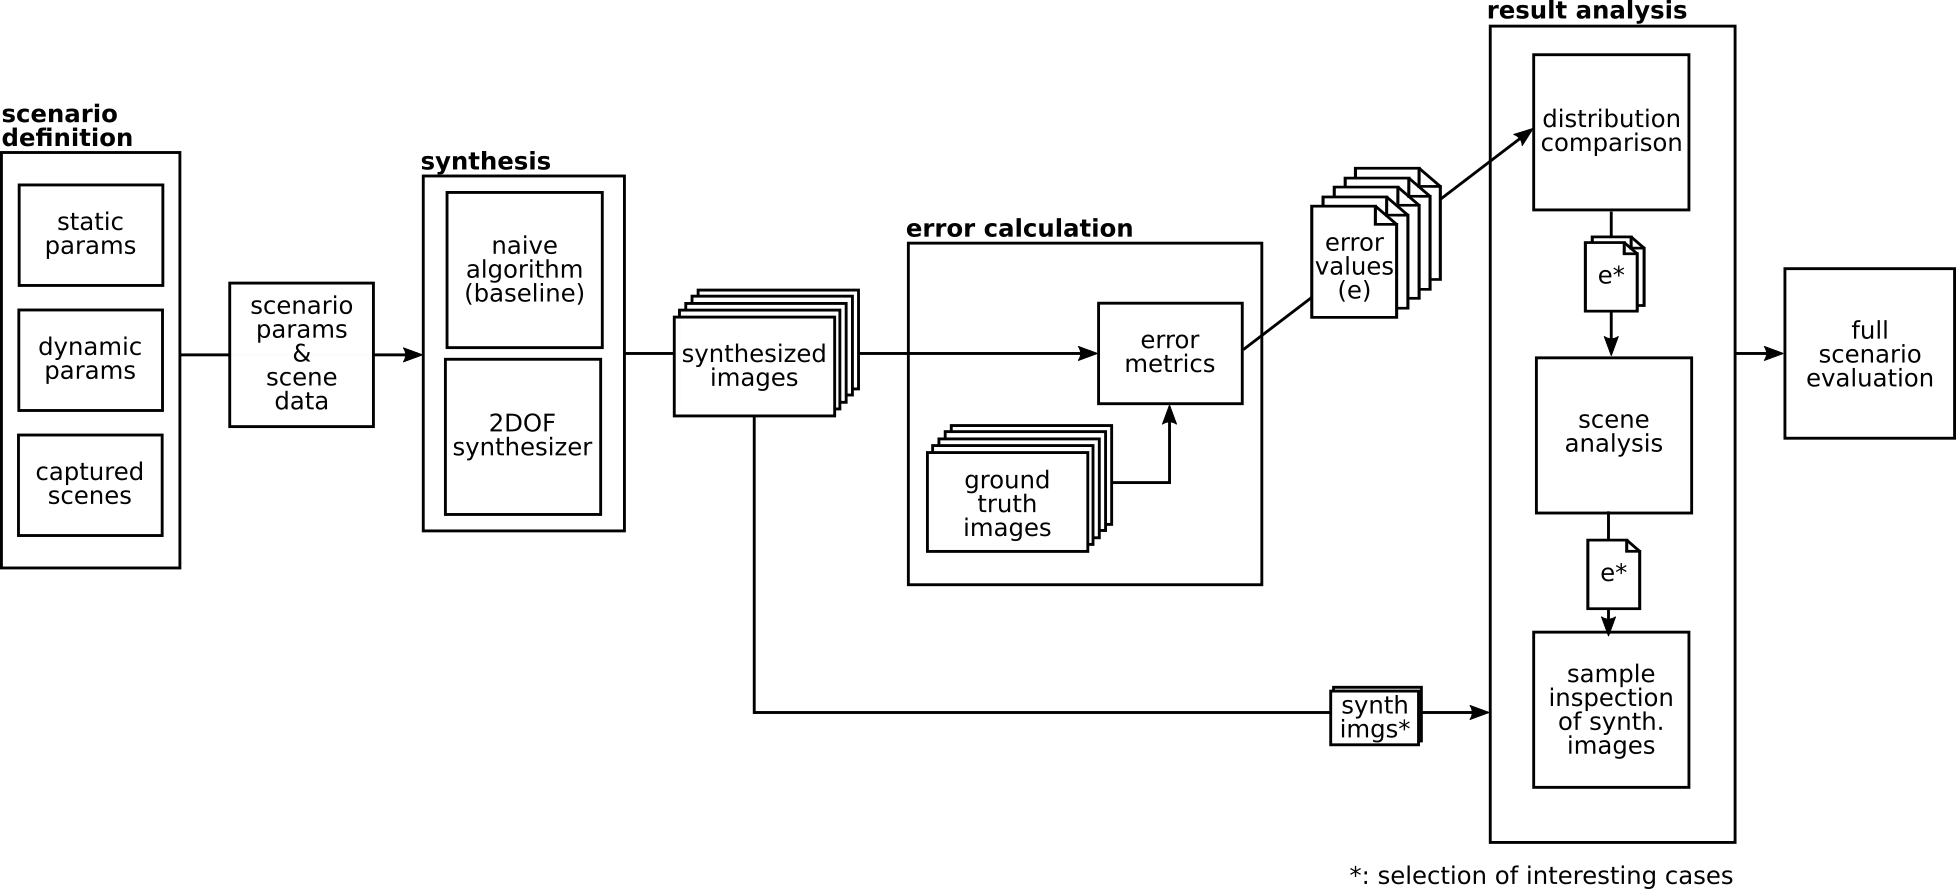
\includegraphics[width=\textwidth]{04/eval_methodology.png}
		\caption{Methodology for the evaluation of a scenario}
		\label{fig:eval-methodology}
\end{figure}

\subsubsection{Scenario Definition}
A scenario is defined by the parameter that it tests, the static parameters that are used, and the scene where the data was captured. Although a scenario is designed to test a specific parameter, which then is ``dynamic'' (i.e., will be modified throughout the scenario), there might also be more dynamic parameters. For example, in a scenario for exploring viewpoint density, the blending type might also be modified to see what effect the viewpoint density has on regular and flow-based blending. The static parameters include the location of the synthesized viewpoints, for example, or any other parameter that remains unchanged throughout the scenario. One other defining factor of a scenario is the scene data that the scenario is tested on. Although the scene is part of the parameters (the external parameters, to be exact), it merits particular mention, as it contains the actual image data that is used for synthesis. This data, along with the other parameters defined in the scenario, are then passed on to the synthesis step.

%First, a scenario must be defined that illustrates the parameter that should be examined. This includes determining which of the parameters should be static, and which should be dynamic. There are two dynamic parameters at maximum, one to be examined, and one to increase the significance of the results. Adding more dynamic parameters per scenario would allow for a more definitive evaluation, but is outside of the scope of this thesis.

%The set of parameters (whether static or dynamic) contains the choice of scene in which to synthesize the images. The scene is defined by its captured viewpoints, metadata, and radius, which are all passed on to the synthesis step along with the other parameters defined for the scenario.

\subsubsection{Synthesis}
The synthesis step consists of three parts: the 2-DoF synthesis presented in Chapter~\ref{chap:implementation} using flow-based blending and regular blending, and a baseline synthesis using a na\"ive algorithm.
The na\"ive algorithm consists of simply selecting the nearest neighbor viewpoint based on euclidean distance. The input parameters are the same for all three algorithms and all the results are passed on to error calculation.
The results of the na\"ive algorithm serve as a baseline comparison to verify whether the developed 2-DoF algorithm is an improvement to a na\"ive approach. If either the regular or the flow-based blending generally performs worse than the na\"ive algorithm, this is an indication of a substantial flaw in the approach.

\subsubsection{Error Calculation}
There are many properties that a synthesis algorithm can be evaluated for, for example execution speed, visual acceptability (based on user studies), number of artefacts, or distance from the ground truth. In this evaluation, mathematical
%In order to evaluate the synthesized images, it is necessary to define metrics with which to measure their accuracy. Since it is outside of the scope of this thesis to evaluate the quality of the results based on human perception, mathematical
error metrics are used to compare each result to its ground truth image. These two metrics, the L1 error and the SSIM error, are chosen since they are based on different image features. As a result, potential limitations of each metric can be compensated for by the other. However, it must be taken into account that neither metric is designed specifically for the task of measuring accuracy of 360\degree synthesized images. As a result, it is necessary to monitor and verify their results by visual examination, especially in cases where the results do not correspond. The details of the L1 and SSIM error metrics are presentented in the following sections.

\paragraph{L1 error on RGB}
The first metric is the L1 error, which is calculated between the ground truth image and the synthesized image in RGB color space. This error metric calculates the mean absolute difference of the RGB values and therefore indicates the mean accuracy of each pixel of the image. 
%The RGB errors of each pixel are added together for the complete image and then divided by the number of pixels in the image. This results in an error value $e_{L1} \in [0,3]$, since the maximum error per pixel is 3 for floating point RGB color values of .
Equation~\ref{eq:l1} shows the formula for the L1 error metric: The difference of the RGB color values $r,g,b \in [0,1]$ (for floating point values) is calculated for each pixel of the ground truth ($P^{gt}$) and synthesized ($P^{s}$) images, then all of the differences are added together, and divided by the number of pixels ($P$) in the image. The range of error values is $e_{L1} \in [0,3]$.

\begin{align}
%  e_{L1} = \frac{1}{|P|} \cdot \sum_{}^{P} \sum_{}^{c \in (r,g,b)} |(c_{gt} - c_{syn})| \label{eq:l1}
  e_{L1} = \frac{1}{|P|} \cdot \sum_{}^{P} |(P_r^{gt} - P_r^{s})| + |(P_g^{gt} - P_g^{s})| + |(P_b^{gt} - P_b^{s})|   \label{eq:l1}
\end{align}


A visualization of the L1 error can also be created by calculating the sum of absolute differences per pixel without averaging the values. Figure~\ref{fig:l1_example} shows an example visualization of the L1 error between two images. The visualization encodes areas of the image where there is a very large difference with a value closer to white and areas where there is no difference as black, which highlights areas of the image that are problematic. Since the sum of the differences between all three color values is used, the visualization can contain oversaturated white areas where the pixel value is larger than 1. Although some information on the severity of the error values is lost due to the oversaturation, problematic areas are more easily recognizable, which is more important for this evaluation.

The L1 error is useful because it gives a rough estimate of how accurately each pixel is synthesized. The visualization indicates in which areas the synthesized image is inaccurate, which is helpful for classifying problems. However, a drawback of the L1 error is that it relies on color values, so images with large differences in pixel values will generally produce a higher error value than images with smaller differences in pixel values, even though the distortion and displacement may be the same.

\begin{figure}
\centering
    \hfill
    \begin{subfigure}[t]{0.3\textwidth}
            \centering
            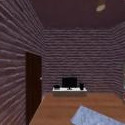
\includegraphics[width=0.9\textwidth]{04/l1_ex01.jpg}
            \caption{}
    \end{subfigure}%
    \hfill
    \begin{subfigure}[t]{0.3\textwidth}
            \centering
            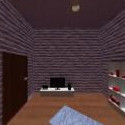
\includegraphics[width=0.9\textwidth]{04/l1_ex02.jpg}
            \caption{}
    \end{subfigure}
    \hfill
    \begin{subfigure}[t]{0.3\textwidth}
            \centering
            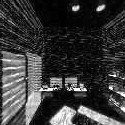
\includegraphics[width=0.9\textwidth]{04/l1_ex03.jpg}
            \caption{L1 error visualization of (a) and (b)}
    \end{subfigure}%
    \hfill
    \hfill
  \caption[Example visualization of L1 RGB error]{Example visualization of L1 RGB error. The RGB error values have been intensified so that they are more visible.} \label{fig:l1_example}
\end{figure}

As in the case of optical flow calculation, some adjustment must be made to adapt this metric for 360\degree images. Since the equirectangular projection is not equal-area, the areas towards the poles would intrinsically have higher weighting, since RGB L1 is calculated per pixel. To avoid this problem, the cube map projection is used, since it does not significantly distort the image. The average value is then calculated using the six faces of the cube.

\paragraph{SSIM error on Grayscale}
The metric to complement the L1 error is a variation of the structural similarity index (SSIM) \cite{ssim}, which measures the \emph{structural similarity} between two images. Instead of comparing the images pixel by pixel, the SSIM uses the luminance, contrast and structure of the images for comparison. It compares these locally, i.e., it operates on smaller areas instead of the image as a whole. Consequently, it is possible that the SSIM does not register small displacements in the scene if the objects are not distorted. However, the additional comparison with the L1 error should mitigate this potential problem.

The SSIM metric in general, and the implementation used in this evaluation\footnote{skimage.metrics.structural\_similarity \cite{skimage}} return a value $SSIM \in [-1, 1]$ with 1 signifying an extremely similar image and -1 signifying a very different image. In order to be able to compare it more easily with the L1 error, the SSIM value is converted to an error value $ e_{SSIM} \in [0,1]$, with 0 signifying an identical image with no error and 1 signifying a very different image.

The SSIM error is calculated on the grayscale image in cubemap representation. There is no need to use an RGB image, since it does not use color values. The cubemap representation is again used to avoid possible problems with distortion.

\subsubsection{Result Analysis}
After calculating the error metrics of all of the synthesized images, the results are analyzed.
For each scenario, the number of results depends on the number of tested parameters and the number of synthesized viewpoints. Furthermore, for each synthesized image, there are two error metrics to be considered. Altogether, this can lead to a very large number of results.
%For each scenario evaluation, one image is synthesized at each selected position using the na\"ive algorithm, the regular blending, and the flow-based blending. The number of images depends on the tested parameters and the number of synthesized viewpoints and each result is measured by the L1 and SSIM error metrics.
%The number of parameters combined with the comparison to the baseline results and the use of two different error metrics results in a large number of error values.
In order to effectively analyze this potentially very large number of results, it is necessary to break the analysis down by creating different visualizations that highlight different attributes of the results. At first, an overview is created, the ``distribution comparison'', from which interesting cases are selected. These cases are examined in more detail using the ``scene analysis'' which shows the results in the context of the scene. Then, exemplary results are selected and inspected visually in the ``sample inspection''. These analysis techniques and their corresponding visualizations are detailed in the following sections.

\paragraph{Distribution Comparison}
The first step of the analysis is a comparison of error value distribution. In order to compare all the error values of a scenario, the values are plotted using a boxplot (Figure~\ref{fig:boxplot_example}). The different parameter combinations of the scenario are plotted on the $y$ axis (e.g., the scene ``square room'') and the error distribution (i.e., the error values of all the synthesized viewpoints) is plotted on the $x$ axis. The box plot shows the distribution of these values: The thick black line in the colored box is the median value (approx. 0.177 in Figure~\ref{fig:boxplot_example}); the colored ranges to the left and right of the median describe the ``interquartile range'' (IQR), the range of the closest half of the data (25\% on each side). The ``whiskers'' of the plot extend to the minimum and maximum of the values. The minimum and maximum are defined as $1.5\cdot IQR$. Any data outside of the range between the minimum and the maximum, are the ``outliers'', depicted as small crosses. The boxplot gives a general overview of how the error values of the specific scene are distrubute. The distribution of the error values of the results in Figure~\ref{fig:boxplot_example}, for example, shows that the first three quartiles of the results are fairly close to the median (between approx. 0.14 and 0.19), whereas the fourth quartile extends, over almost the same range (0.19 to 0.225) and there are some extreme outliers. This indicates that there are some viewpoints that performed significantly worse than most of the others.

\paragraph{Scene Analysis}
Based on the insights gained in the distribution comparison, the most interesting cases are selected for closer analysis. These cases are examined by color coding the error values and assigning the colors to the positions in the scene. This puts the error values in context with the scene surroundings. In the example distribution visualization in Figure~\ref{fig:boxplot_example}, there is only one scene, so the choice is trivial: Figure~\ref{fig:posmap_example} shows the synthesized points in the context of this ``square room'' scene, color coded by their error values. The maximum and minimum values of the points (also clearly visible in Figure~\ref{fig:boxplot_example}) are coded as light green and dark blue, respectively. This visualization gives a more detailed overview over the values of the different points. In Figure~\ref{fig:posmap_example}, for example, the synthesized points near the right wall of the room have much better (i.e., lower) values than the row on the left side of the room. The four light green values are clearly the outliers that were visible in Figure~\ref{fig:boxplot_example}. Using this information, it is possible to draw some conclusions about the effect of the position of the synthesized viewpoint relative to the objects in the scene, and select a few synthesized images that merit closer examination.

\begin{figure}
\centering
    \hfill
    \begin{subfigure}[c]{0.5\textwidth}
            \centering
            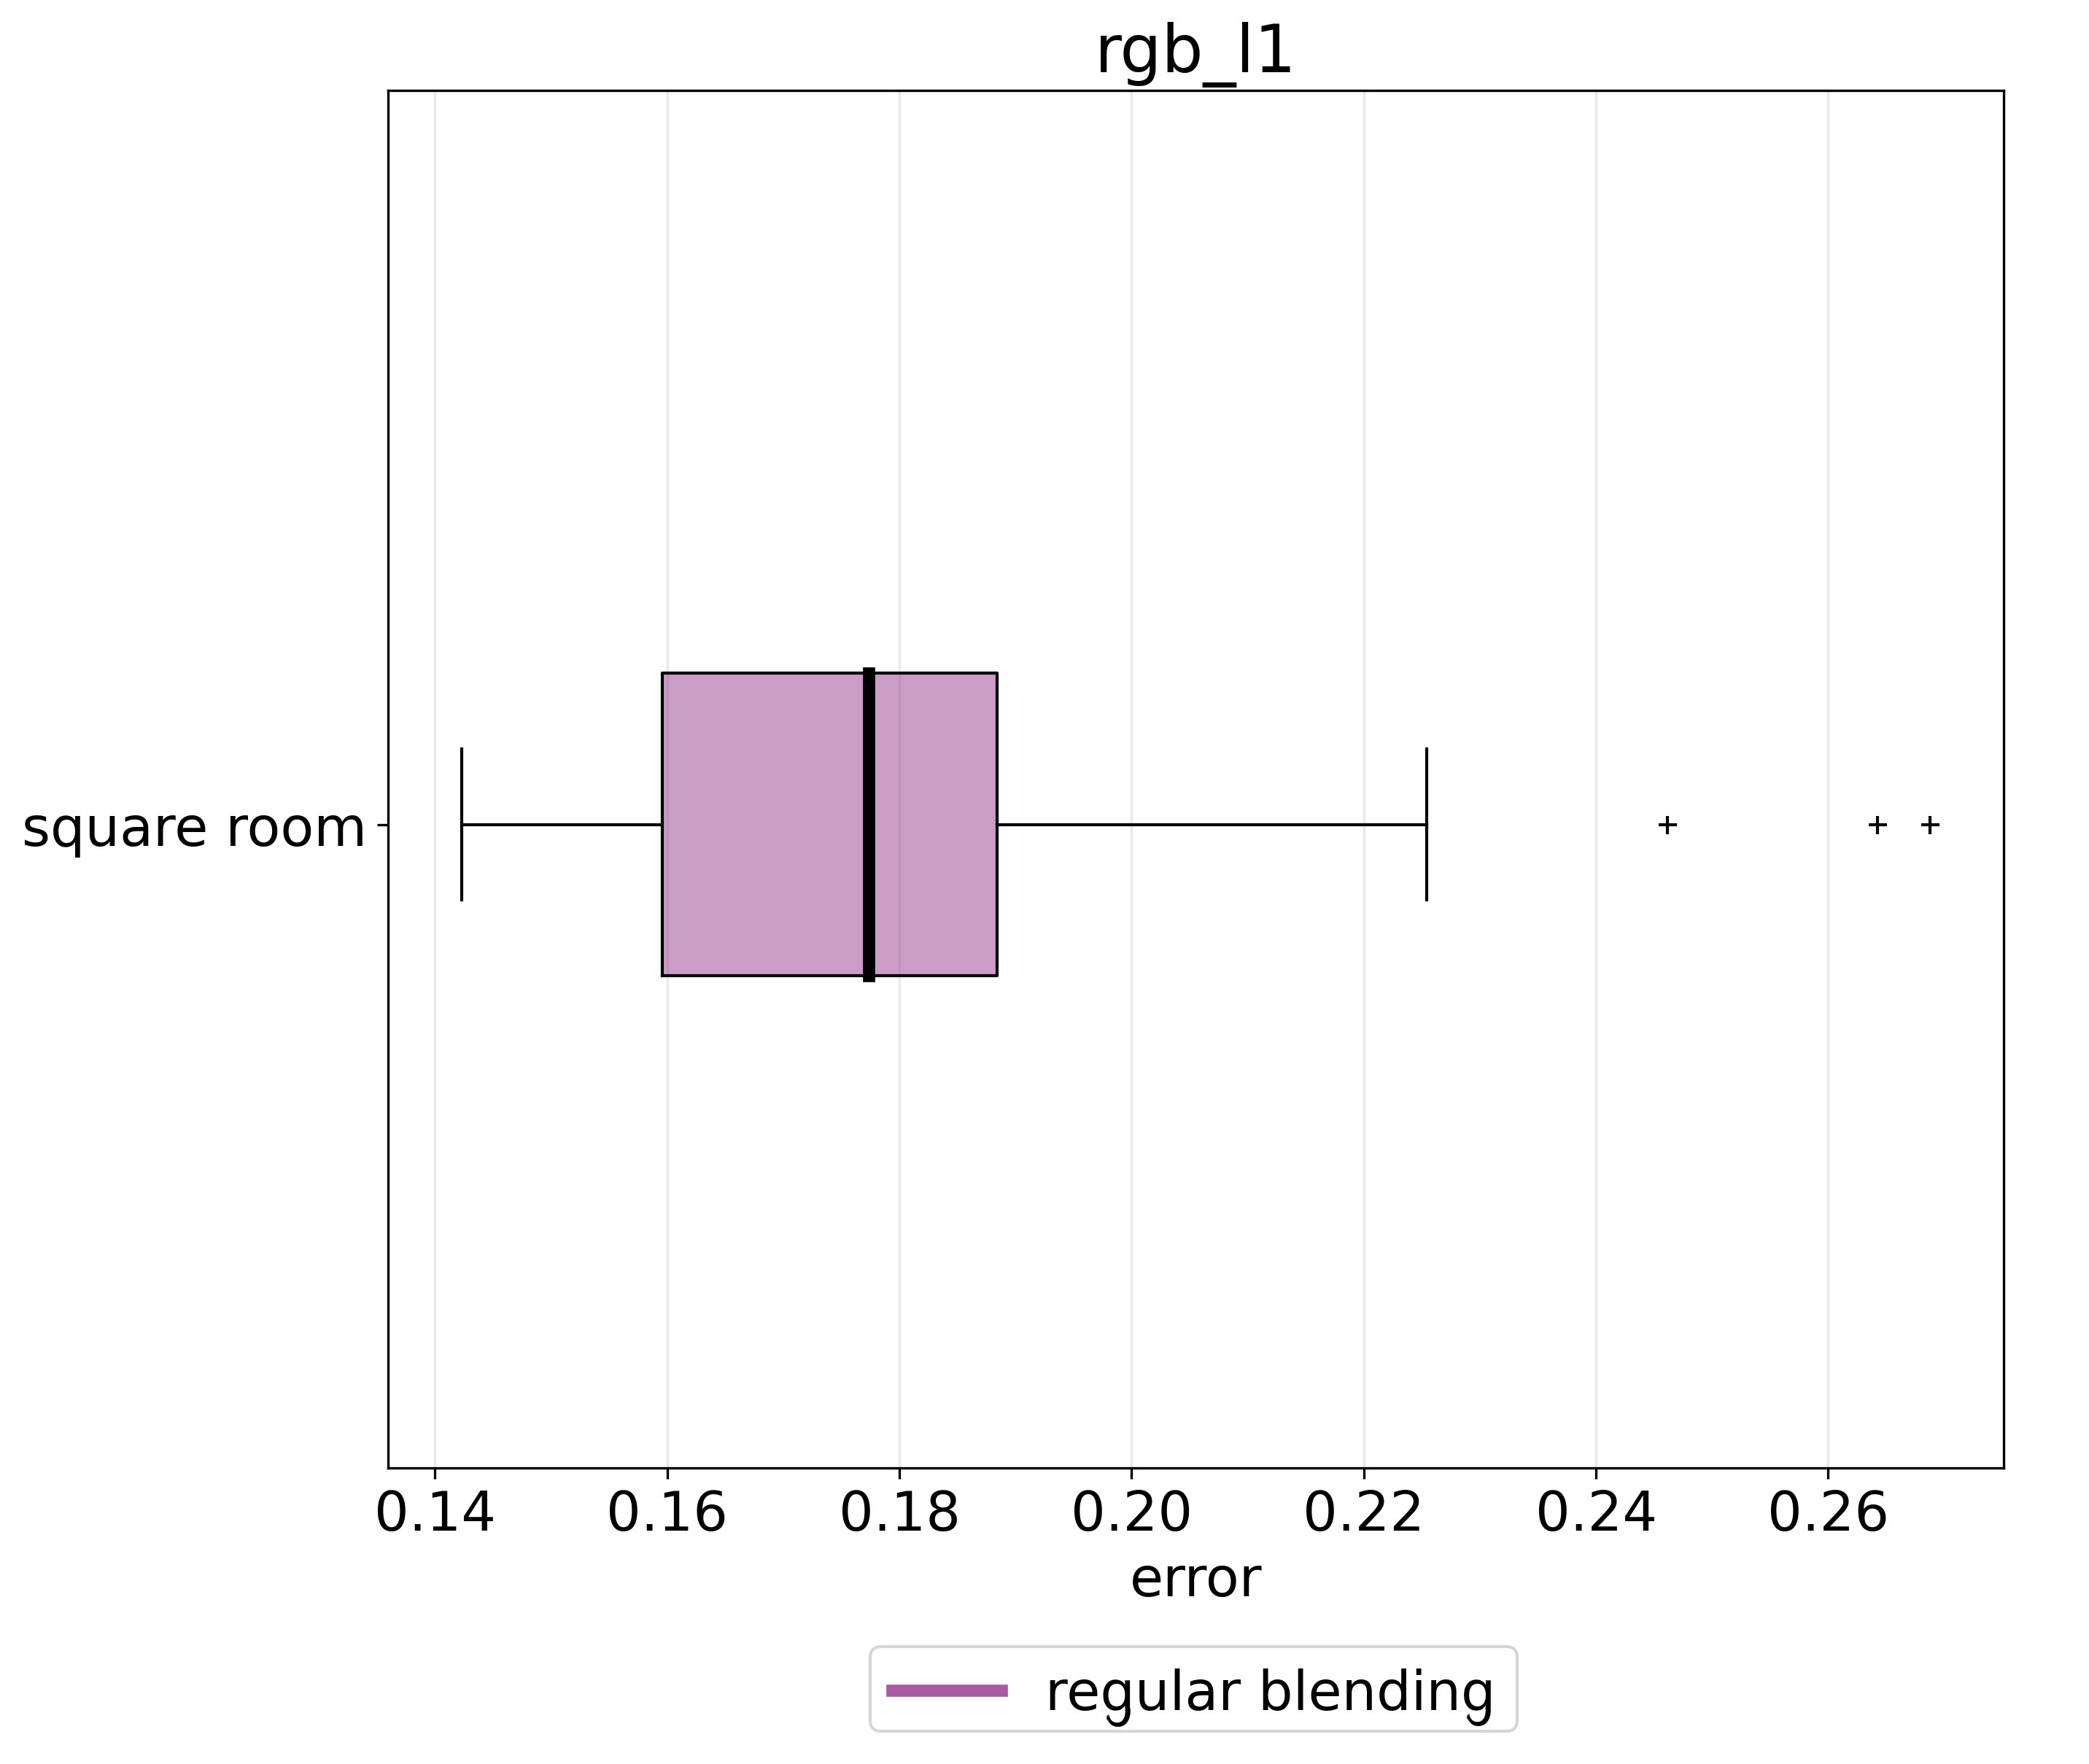
\includegraphics[height=6cm]{04/boxplot_example.jpg}
            \caption{Boxplot example for distribution comparison of the results of regular blending in the ``square room''} \label{fig:boxplot_example}
    \end{subfigure}%
    \hfill
    \begin{subfigure}[c]{0.5\textwidth}
            \centering
            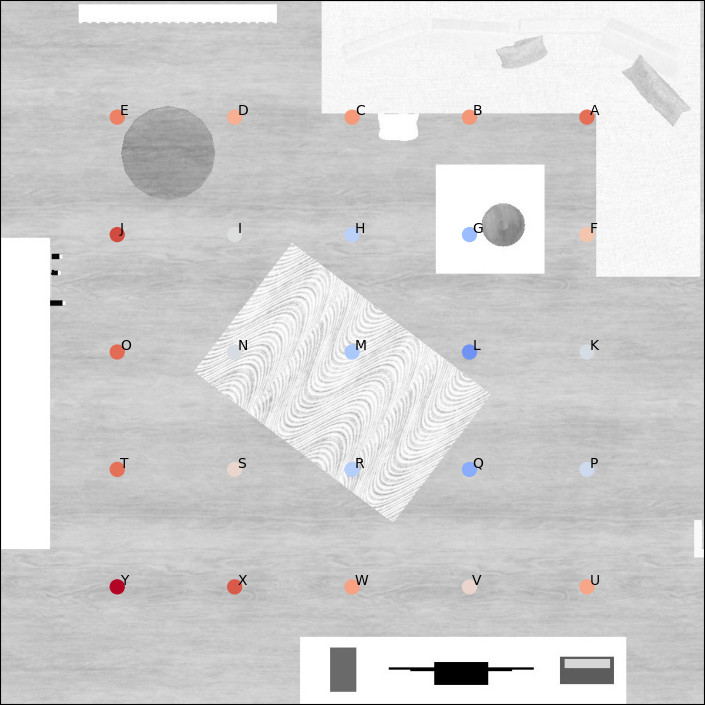
\includegraphics[height=6cm]{04/posmap_example.png}
            \caption{Visualization for scene analysis: The error values from the boxplot in (a) are mapped to colors at the positions of the viewpoints in the scene. Light green represents the worst value (0.268) and dark blue the best value (0.143).} \label{fig:posmap_example}
    \end{subfigure}
    \hfill
  \caption[Different types of result visualizations for L1 error values]{Different types of result visualizations for L1 error values for example results of regular blending in a scene}
\end{figure}

\paragraph{Sample Inspection}
In order to further understand the effects of the parameters on specific positions, some of the synthesized viewpoints from the scene analysis are examined visually by comparing the synthesized image to the ground truth image. The visual examination may also reveal information that the error metrics are unable to extract, such as specific types of artefacts. For example, by using the information presented in Figure~\ref{fig:posmap_example}, it is possible to choose one of the best results, for example synthesized point ``K'' near the right wall in the middle. The close inspection of the synthesized images is shown in Figure~\ref{fig:inspection_example}: In the left column from top to bottom are the ground truth image, the synthesized image using regular blending, and the synthesized image using flow-based blending. In the right column are the L1 difference images to the ground truth image. They can help with understanding the error values. For example, the accuracy of the rug in the bottom face (marked in green) is improved in the flow result compared to the regular result in Figure~\ref{fig:inspection_example}. However, the flow result also has a fairly large artefact at the top of the door in the left face (magenta ring), which is not the case in the regular result.
%\footnotetext{The synthesized images are shown in Appendix~\ref{imgs}, in order to avoid interrupting the flow of the text, since they take up a fairly large amount of space.}

\begin{figure}
		\centering
		\includegraphics[width=\textwidth]{04/inspection_example_K.jpg}
		\caption[Sample inspection of viewpoint ``K'']{Sample inspection of example viewpoint ``K'': The images are in cube map representation, as this is tends to be more intuitive to understand than latlong representation. Depending on the content, different faces may be omitted.}
		\label{fig:inspection_example}
\end{figure}
















\section{Parameter Evaluation Using Virtual Scenes} \label{sec:limit_eval}
In the first part of the evaluation, virtual scenes are used to evaluate the performance of the 2-DoF synthesis using regular blending and flow-based blending with different parameters.
Virtual scenes allow full control over the external parameters, for example the scene geometry, and the positions of the captured and synthesized viewpoints, as well as enabling automatic generation of the images at the chosen positions.
As a result, it is possible to test setups that would be unfeasible for real scenes, for example setups using a large number of captured viewpoints at varying locations in different scenes.
The following three scenarios are tested using virtual scenes:
\begin{description}
\item [``Different Scene Geometries''] This scenario tests the effect of various scene geometries on the results. This includes the \emph{basic shape} of the scene as well as the \emph{objects within the scene}.
\item [``Density of Captured Viewpoints''] This scenario tests the effect of the \emph{density} of the captured viewpoints on the results. The density of the viewpoints is defined by how closely together the viewpoints are captured throughout the scene.
\item [``Position of Synthesized Viewpoints Relative to Captured Viewpoints''] This scenario tests the effect of the \emph{relative position} of a synthesized viewpoint \emph{compared to the captured viewpoints}, for example how close a synthesized viewpoint is to a captured viewpoint.
\end{description}

%The selected internal and external parameters that will be explored in the scenarios tested in the virtual scenes are:
%\begin{itemize}
%  \item proxy-scene difference (how dissimilar is the scene geometry from the proxy sphere geometry, including the objects within the scene)
%  \item density of the captured viewpoints
%  \item position of the synthesized viewpoints relative to the captured viewpoints
%%  \item flow-based blending compared to regular blending
%\end{itemize}

%A scenario is designed for each of the three parameters, containing several different setups to test the performance and limitations of the algorithm developed in Section~\ref{chap:implementation}. 

The virtual scenes used in the scenarios are presented in Section~\ref{subsec:data_acquisition}, and the method of obtaining optical flow for these scenes is described in Section~\ref{subsec:gt_of}. Then, in Section~\ref{subsec:virt_results}, the setup of each scenario is described in detail, and the results of the evaluation of each scenario are presented and discussed. Finally, the insights from the evaluations of all of the scenarios are summarized and discussed in Section~\ref{subsec:discussion_virtual}.
%Using the generated scenes and optical flow, as well as the parameters defined for this evaluation, it is now possible to design, test, and evaluate the following scenarios:


\subsection{Data Acquisition and Featured Scenes} \label{subsec:data_acquisition}
%In order to be able to test these scenarios, it is necessary to generate appropriate scenes. However, the manual capture of viewpoints as well as ground truth data can be very time-consuming. Furthermore, since locations need to be recorded either by hand, or calculated by a structure-from-motion algorithm or something similar, it is possible that the final locations are not perfectly accurate. In order to circumvent these problems, virtual scenes are used for the evaluation of limits. 


Three different virtual scenes are employed for the scenarios, modeled using the animation software Blender \cite{blender}: the \emph{checkersphere}, the \emph{square room} and the \emph{oblong room}.% and the \emph{oblong room II}.

\paragraph{Checkersphere}
The \emph{checkersphere} (Figure~\ref{fig:checkersphere}) is a perfect sphere with a radius of approximately 2m. Its surface is covered with a checkerboard pattern with alternating colors of dark blue, dark red, and dark green.
%It represents a scene where the geometry of the scene is exactly the same as the proxy geometry.
Although this kind of room is not likely to exist in reality, it represents an interesting case, since the scene geometry is identical to the proxy geometry. The checkerboard pattern is chosen so that distortions or inaccuracies are more visible.

\begin{figure}[p]
\centering
    \hfill
    \begin{subfigure}[t]{0.7\textwidth}
            \centering
            \includegraphics[height=5cm]{04/checkersphere_overview.jpg}
            \caption{Latlong image from the center of the sphere}
    \end{subfigure}%
    \hfill
    \begin{subfigure}[t]{0.3\textwidth}
            \centering
            \includegraphics[height=5cm]{04/checkersphere_outside.jpg}
            \caption{View from the outside for reference}
    \end{subfigure}
    \hfill
  \caption{Overview of the ``checkersphere''}
  \label{fig:checkersphere}
\end{figure}

\begin{figure}[p]
\centering
    \hfill
    \begin{subfigure}[b]{0.7\textwidth}
            \centering
            \includegraphics[height=5cm]{04/square_overview.jpg}
            \caption{Latlong image from the center of the room}
    \end{subfigure}%
    \hfill
    \begin{subfigure}[b]{0.3\textwidth}
            \centering
            \includegraphics[height=5cm]{04/square_top.jpg}
            \caption{Top view}
    \end{subfigure}
    \hfill
  \caption{Overview of the ``square room''}
  \label{fig:square_room}
\end{figure}

\begin{figure}[p]
\centering
    \hfill
    \begin{subfigure}[b]{0.7\textwidth}
            \centering
            \includegraphics[height=5cm]{04/oblong_overview.jpg}
            \caption{Latlong image from the center of the room}
    \end{subfigure}%
    \hfill
    \begin{subfigure}[b]{0.3\textwidth}
            \centering
            \includegraphics[width=5cm]{04/oblong_top.jpg}
            \caption{Top view}
    \end{subfigure}
    \hfill
  \caption{Overview of the ``oblong room''}
  \label{fig:oblong_room}
\end{figure}

\paragraph{Square Room}
The \emph{square room} (Figure~\ref{fig:square_room}) is a room whose basic shape is a perfect cube with a side length of 3.5m. It contains an assortment of furniture\footnotemark: In one corner, there is an orange, L-shaped couch with dark blue and white cushions on it. In front of the couch is a small, white marble coffee table with a dark blue bowl on it. Several small, simple black and white pictures are hanging on the wall behind the couch. There is a blue and white rug in the middle of the room, and to the left of the couch are a round blue table, as well as a white radiator. On the wall next to the blue table is a white marble bookshelf containing several red books, as well as three wine bottles, and two decorational objects in green and purple. Across from the couch is a low marble TV cabinet carrying a black monitor, a black laptop and a black speaker. To the left of the cabinet is a wooden door with a gray handle. The walls are brick, painted a dark purple, and there is a lamp with a white lampshade hanging from the middle of the ceiling.
\footnotetext{The furniture models used in the square room and the oblong room are adapted from \url{https://www.cgtrader.com/free-3d-models/interior/living-room/low-poly-interior-57731178-c955-4625-9e44-109c8eea5ee2}, by user ``miha29076'', and the textures are adapted from \url{https://www.poliigon.com/texture/plaster-17}, \url{ https://www.poliigon.com/texture/fabric-denim-003}, \url{https://www.poliigon.com/texture/wood-fine-dark-004}, and \url{https://www.poliigon.com/texture/interior-design-rug-starry-night-001}. \emph{All accessed last on September 23, 2020}}

The purpose of using the square room is to have a basic shape that is similar to the proxy sphere geometry, while at the same time offering a more realistic indoor setting.

\paragraph{Oblong room}
The \emph{oblong room} (Figure~\ref{fig:oblong_room}) has a room size of approximately 5.5m x 3.5m and contains the same basic elements as the square room. It has the exact same furniture layout as the square room, except that the basic shape of the room is different. The walls are dark blue, instead of dark purple, in order to be able to differentiate between the square and oblong rooms at a glance.

\begin{figure}
\centering
    \hfill
    \begin{subfigure}[b]{0.4\textwidth}
            \centering
            \includegraphics[width=0.9\textwidth]{04/vps_checkersphere.jpg}
            \caption{The captured viewpoints in the checkersphere}
    \end{subfigure}
    \hfill
    \begin{subfigure}[b]{0.4\textwidth}
            \centering
            \includegraphics[width=0.9\textwidth]{04/vps_square.jpg}
            \caption{The captured viewpoints in the square room}
    \end{subfigure}
    \hfill
    \hfill

    \hfill
    \begin{subfigure}[b]{0.4\textwidth}
            \centering
            \includegraphics[width=0.9\textwidth]{04/vps_oblong.jpg}
            \caption{The captured viewpoints in the oblong room}
    \end{subfigure}
    \hfill
    \hfill
  \caption[The grid of captured viewpoints in each scene, including the proxy geometry]{The grid of captured viewpoints in each scene, including the proxy geometry as a gray circle. The scene sizes are not to scale.} \label{fig:vps_grid}
\end{figure}

\paragraph{}
Since the results of the different scenes are compared, it is necessary to choose comparable captured viewpoints, since these are used as input for the synthesis. Since the scenes all have similar scale, the viewpoint layout is chosen to be identical in all of the scenes: All scenes contain 36 captured viewpoints, aligned in a regular grid of 6x6 viewpoints, with 60cm spacing. The grid of viewpoints is centered within the scene. This means that in the checkersphere (Figure~\ref{fig:vps_grid}a) and the square room (Figure~\ref{fig:vps_grid}b), the viewpoints cover approximately the complete scene, and in the oblong room there is about a 1m area on each side of the grid that is not covered (Figure~\ref{fig:vps_grid}c). It is necessary to take this difference in viewpoint coverage into account for the evaluation, since the viewpoints in the oblong room have a larger distance to two of the walls, which may have an effect on the accuracy of the results.

Since Blender is designed for creating animated movies, and not the capture of static viewpoints, some adjustments have to be made to be able to capture the chosen viewpoints as well as the ground truth images: After choosing the positions of the input viewpoints for the scenes, the position of the camera for each captured viewpoint is stored as a keyframe, so that the batch of viewpoints can be rendered like an animation. A Blender script is used in order to automatically assign the viewpoints and the ground truth points to the keyframes, and write out the metadata. This way the locations of the viewpoints are always be perfectly accurate, and the ``capture'' of the viewpoints requires no manual effort. The images are rendered with a resolution of 1000x500 for all of the scenes, in order to reduce the computation time for the image synthesis in the tests.




\newpage
\subsection{Synthesizing Optical Flow with Blender} \label{subsec:gt_of}
Using Blender to create virtual scenes not only facilitates capture, but also offers an alternative to calculating optical flow. As mentioned in Section~\ref{subsec:optical_flow}, most optical flow algorithms struggle with large displacements.
The flow-based blending step in the 2-DoF synthesis algorithm, on the other hand, assumes acceptably accurate optical flow and there is no attempt to judge whether the optical flow calculation is feasible between two selected viewpoints.
As a result, given the wrong circumstances (two viewpoints A and B that are far apart), the optical flow algorithm may fail, leading the flow-based blending to output undesirable results. The success of the optical flow algorithm is a prerequisite for the success of the 2-DoF algorithm with flow-based blending.

Contrarily, the focus of this evaluation is not the accuracy of an arbitrary optical flow algorithm. In the best case, it would be possible to emulate ``perfect'' optical flow, thus decoupling the success of the optical flow from the success of the flow-based blending. While this is practically impossible for real scenes, virtual scenes theoretically contain all necessary information for retrieving ``ground truth'' optical flow. Blender, for example, is capable of ``rendering'' motion vectors using its vector speed render pass, which calculates the movement between points from one frame to the next in pixel space. The result is a motion vector field, which corresponds to the result of a ``classic'' optical flow algorithm. This ``ground truth'' optical flow (in the optimal case) was first presented by Butler et al.\ \cite{sintel} as a benchmark for optical flow algorithms.

In order to demonstrate the improvement of Blender optical flow compared to Farneb\"ack optical flow, which is the optical flow algorithm used in the implementation, a small scene setup is tested using 1-DoF interpolation. Figure~\ref{fig:of_comparison}a shows the test setup: 25 viewpoints are interpolated at the interpolation distance $\delta = 0.5$ between captured points. Each of the 25 viewpoints is interpolated twice: Once using Farneb\"ack optical flow, and once using Blender optical flow. The results of both interpolations are then compared using the error metrics.
Figure~\ref{fig:of_comparison}b shows the improvement of the results using Blender optical flow: In all but one case for the L1 values, and in the majority of the SSIM values, the Blender optical flow improves the error values, shown by the positive values in Figure~\ref{fig:of_comparison}b. Visually, the improvement by using Blender optical flow is clear: Figure~\ref{fig:of_comparison}c shows the viewpoint ``I'' interpolated using Farneb\"ack optical flow, and Figure~\ref{fig:of_comparison}d the same viewpoint using Blender optical flow. There are distincly fewer artefacts with Blender optical flow, for example the rug and the couch both have a much more distinct outline, and the bookshelf is also clearer. Figure~\ref{fig:of_comparison}e and Figure~\ref{fig:of_comparison}f show the same for interpolated viewpoint ``M''. In this case, the TV cabinet and the rug are much clearer in the Blender optical flow version (Figure~\ref{fig:of_comparison}f).

\begin{figure}
\centering
    \hfill
    \begin{subfigure}[c]{0.4\textwidth}
            \centering
            \includegraphics[width=0.9\textwidth]{04/gt_flow/1DoF_scene.png}
            \caption{The interpolated viewpoints A-Y (in orange) for testing optical flow}
    \end{subfigure}
    \hfill
    \begin{subfigure}[c]{0.4\textwidth}
            \centering
            \includegraphics[width=0.9\textwidth]{04/gt_flow/blender_flow_improvement_small.png}
            \caption{The improvement of error values using Blender optical flow vs Farneb\"ack optical flow. Here, a positive value signifies a reduction of the error value.}
    \end{subfigure}
    \hfill
    \hfill
\par\bigskip
    \hfill
    \begin{subfigure}[b]{0.4\textwidth}
            \centering
            \includegraphics[width=0.9\textwidth]{04/gt_flow/I_calcflow.jpg}
            \caption{1-DoF interpolated viewpoint ``I'' using Farneb\"ack optical flow}
    \end{subfigure}
    \hfill
    \begin{subfigure}[b]{0.4\textwidth}
            \centering
            \includegraphics[width=0.9\textwidth]{04/gt_flow/I_blenderflow.jpg}
            \caption{1-DoF interpolated viewpoint ``I'' using Blender optical flow}
    \end{subfigure}
    \hfill
    \hfill
\par\bigskip
    \hfill
    \begin{subfigure}[b]{0.4\textwidth}
            \centering
            \includegraphics[width=0.9\textwidth]{04/gt_flow/M_calcflow.jpg}
            \caption{1-DoF interpolated viewpoint ``M'' using Farneb\"ack optical flow}
    \end{subfigure}
    \hfill
    \begin{subfigure}[b]{0.4\textwidth}
            \centering
            \includegraphics[width=0.9\textwidth]{04/gt_flow/M_blenderflow.jpg}
            \caption{1-DoF interpolated viewpoint ``M'' using Blender optical flow}
    \end{subfigure}
    \hfill
    \hfill
  \caption[Comparing 1-DoF interpolation results using calculated vs Blender optical flow]{Comparing 1-DoF interpolation results using Farneb\"ack to results using Blender optical flow} \label{fig:of_comparison}
\end{figure}

%\begin{figure}
%		\centering
%		\includegraphics[width=\textwidth]{04/blender_flow_improvement.png}
%		\caption[Accuracy improvement with Blender flow versus Farneb\"ack flow]{Accuracy improvement with Blender flow versus Farneb\"ack flow: The y axis shows the improvement of the error metric when using Blender flow.}
%		\label{fig:calc_vs_synth_flow}
%\end{figure}

It is notable that using Blender optical flow tends to improve the results compared to Farneb\"ack's algorithm, but that does not mean that the resulting optical flow is completely accurate. For example, the bookshelf in the right and middle faces in Figure~\ref{fig:of_comparison}d still shows warping and doubling effects, indicating that there are still some inaccuracies. The same is true for the coffee table and the blue round table in the bottom face. There are several possible reasons for this, mostly based on the fact that the process in Blender, like most optical flow algorithms, is designed for frame-to-frame use, and has in this case been ``misused'' for movements between frames that are unrealistic for an actual animation. Nevertheless, no definitive explanation can be made at this point, since this would require in-depth understanding of Blender's vector speed render pass, which is outside of the scope of this thesis. Based on the results shown in Figure~\ref{fig:of_comparison}, and experience gained from testing both variants, the Blender optical flow is used for the tests, because, even though it is not completely accurate, it still seems to mostly yield better results than Farneb\"ack's optical flow algorithm and as such decouples (to a degree) the success of the synthesis with flow-based blending from the success of the optical flow algorithm.

%\begin{itemize}
%   \item points that are not visible because of perspective shift will not have a correspondence
%   \item distortion due to wide fov may have an effect on the results
%   \item even blender motion vectors are for frame to frame use, so it is possible, that large jumps do not work well because the blender algo can't handle it
%\end{itemize}

\subsection{Scenarios and Results}\label{subsec:virt_results}
Using the generated scenes and optical flow, it is now possible to test and evaluate the scenarios ``Different Scene Geometries'', ``Density of Captured Viewpoints'' and ``Position of Synthesized Viewpoints Relative to Captured Viewpoints''. 
%\begin{itemize}
%  \item ``Different Scene Geometries''
%  \item ``Density of Captured Viewpoints''
%  \item ``Position of Synthesized Viewpoints Relative to Captured Viewpoints''
%\end{itemize}
For each scenario, the scenes, viewpoint setups, and tested parameters are presented. Then, the \emph{regular blending results} (i.e., the results of the synthesis using regular blending) are discussed, followed by the \emph{flow-based blending results} (i.e., the results of the synthesis using flow-based blending). Next, the flow-based blending results are compared to the regular blending results in order to determine whether the synthesis using flow-based blending performs better than the synthesis using regular blending in the given scenario. Finally, the results of the scenario evaluation are summarized.
%in each of these scenarios, as well as the results of the tests, which are evaluated using distribution comparison, scene analysis, and sample inspection, as described in Section~\ref{sec:eval_methodology}. First the effect of the tested parameter on the regular blending results is examined, then the effect on the flow-based blending results is examined, and 

\subsubsection{Scenario 1: Different Scene Geometries}
The first parameter to be examined is the effect of different scene geometries on the accuracy of the results. There are two different attributes of scene geometry that may have an influence on the result: the basic shape of the scene (e.g., sphere, cube, rectangular prism, or arbitrary polygon), and the objects within the scene. Both of these attributes are considered in the evaluation. All the scenes presented in \ref{subsec:data_acquisition} are used for testing, as they differ both in their basic shape, as well as in the arrangement of the objects within, although the square room and the oblong room are more similar to each other than to the checkersphere.
%A key factor of this scenario is how different the scenes are from the proxy geometry. The larger the difference, the more inaccurate the result of the reprojection will be.

The arrangement of captured viewpoints in all the scenes is identical (a 6x6 grid with a spacing of 60cm), and 25 viewpoints are synthesized in each scene (Figure~\ref{fig:scene_setup}). The synthesized points are near the center or in the center of each grid cell, since these are the areas where the deviation angles are the highest, and where the largest artefacts for the regular blending are expected to emerge. In the square and oblong rooms, the synthesized points are slightly offset from the center of each grid cell.
This offset is necessary in order to test actual 2-DoF synthesis, instead of just 1-DoF interpolation, since synthesizing a viewpoint in the center of a grid cell could be done with only 1-DoF interpolation (e.g., by interpolating by 0.5 between the top right to the bottom left captured viewpoint, as was done in Section~\ref{subsec:gt_of} for testing Blender optical flow). No offset is used in the checkersphere scene, since the checkersphere scene is expected to have excellent results for the regular blending (since the proxy geometry and scene geometry are identical). In this case it is more interesting to use one of the presumably best positions for the flow-based blending to see how well it holds up in comparison.

\begin{figure}
\centering
    \hfill
    \begin{subfigure}[b]{0.4\textwidth}
            \centering
            \includegraphics[width=\textwidth]{04/scenario_scene/sphere_points.jpg}
            \caption{The checkersphere}
    \end{subfigure}%
    \hfill
    \begin{subfigure}[b]{0.4\textwidth}
            \centering
            \includegraphics[width=\textwidth]{04/scenario_scene/square_points.jpg}
            \caption{The square room}
    \end{subfigure}
    \hfill
    \hfill

    \hfill
    \begin{subfigure}[b]{0.4\textwidth}
            \centering
            \includegraphics[width=\textwidth]{04/scenario_scene/oblong_points.jpg}
            \caption{The oblong room}
    \end{subfigure}%
    \hfill
%    \begin{subfigure}[b]{0.4\textwidth}
%            \centering
%            \includegraphics[width=\textwidth]{04/scenario_scene/oblong2_points.jpg}
%            \caption{The oblong room II}
%    \end{subfigure}
%    \hfill
    \hfill
  \caption[The captured and synthesized viewpoints in the different scenes]{The captured (blue) and synthesized (orange) viewpoints in the different scenes (scenes are not to scale)} \label{fig:scene_setup}
\end{figure}

\begin{figure}
\centering
    \hfill
    \begin{subfigure}[b]{0.49\textwidth}
            \centering
            \includegraphics[width=\textwidth]{04/scenario_scene/boxplot_regular.png}
            \caption{Regular blending}
    \end{subfigure}
    \hfill
    \begin{subfigure}[b]{0.49\textwidth}
            \centering
            \includegraphics[width=\textwidth]{04/scenario_scene/boxplot_flow.png}
            \caption{Flow-based blending}
    \end{subfigure}
    \hfill
  \caption{Comparing the distributions of the results in different scenes}
  \label{fig:scene_boxplot_split}
\end{figure}

\paragraph{Regular Blending Results}
The boxplot in Figure~\ref{fig:scene_boxplot_split}a shows the distributions of the error values for the regular blending results in the three scenes. The most striking feature of this distribution is that the checkersphere results show the highest error values for the L1 error, whereas they show the lowest values for the SSIM error. At first, this seems surprising, both because the error metrics do not ``agree'', as well as because the results of the regular blending are expected to be very good since the scene geometry is identical to the proxy geometry. The reason for the comparatively high L1 values is the sensitivity of the L1 metric to different color values. L1 errors on the images of the checkersphere will generally produce a higher value than in other scenes because of the checkerboard texture:
The difference between a dark blue pixel of a dark checkerboard field, and a white pixel on a white checkerboard field is close to 1, whereas the difference between a dark brown pixel and a dark purple pixel (e.g., between the door and the wall in one of the rooms) will produce a lower error value, although the distortion or displacement may be identical. The SSIM error metric, which does not take the color values of the pixels into account, produces a distribution that is much closer to the expected result: Since the scene geometry is identical to the proxy geometry, the result of the reprojection should be almost perfect. And in fact, when visually comparing the results of a synthesized viewpoint to the ground truth (Figure~\ref{fig:scene_checkersphere_Y}), the only difference is a little bit of blurriness due to sampling differences. The white lines in the L1 difference depicted in the right column of Figure~\ref{fig:scene_checkersphere_Y} show how the blurriness caused the high L1 error.

\begin{figure}
		\centering
    \includegraphics[width=\textwidth]{04/scenario_scene/stripX_checkersphere_Y.jpg}
		\caption[Viewpoint ``Y'' in the checkersphere]{Results for synthesized viewpoint ``Y'' in the checkersphere: The regular blending result is very close to the ground truth, except for some blurriness. The flow-based blending result shows some inaccuracies (magenta) and noise (green)}
		\label{fig:scene_checkersphere_Y}
\end{figure}

\begin{figure}
\centering
    \hfill
    \begin{subfigure}[b]{0.4\textwidth}
            \centering
            \includegraphics[width=\textwidth]{04/scenario_scene/01_square__regular.png}
            \caption{Error values of regular blending in the square room}
    \end{subfigure}
    \hfill
    \begin{subfigure}[b]{0.4\textwidth}
            \centering
            \includegraphics[width=\textwidth]{04/scenario_scene/01_oblong__regular.png}
            \caption{Error values of regular blending in the oblong room}
    \end{subfigure}
    \hfill
  \caption[Scene analysis visualization of regular blending results in the square and oblong rooms]{Scene analysis visualization of regular blending results in the square and oblong rooms. Higher values indicate ``worse'' accuracy and lower values indicate ``better'' accuracy.} \label{fig:scene_regular_square_oblong}
\end{figure}

The trend of the error metrics of the other two rooms is consistent: Both the L1 and SSIM error values of the square room are generally higher than those of the oblong room. In this case, comparing the RGB color values is more reliable, since both rooms use the same textures. The results however, are surprising: Although the basic geometry of the square room is closer to the proxy geometry, the error values in the square room are generally higher than those in the oblong room.
A closer scene analysis shows the likely reason for this: The scene analysis visualization of the square room in Figure~\ref{fig:scene_regular_square_oblong}a shows that the error values are particularly high near the bookshelf on the left side of the room, whereas in the oblong room (Figure~\ref{fig:scene_regular_square_oblong}b) the values on the left side of the room are very low and the bookshelf is farther away from the viewpoints.
In order to find out whether the position of the bookshelf is the reason for this drastic difference, the synthesized images at location O (closest to the bookshelf) for the two scenes (Figure~\ref{fig:scene_O_regular}) are inspected. The inspection confirms this presumption: The bookshelf is so close to viewpoint O in the square room, that there are extreme inaccuracies in the synthesis due to large deviation angles. In the oblong room, the bookshelf is much further away, making the devation angles much smaller and the result more accurate. The larger net distance to the walls and some of the objects in the oblong room is the likely reason for the lower error results throughout the scene.

\begin{figure}
		\centering
    \includegraphics[width=\textwidth]{04/scenario_scene/O_regular_both_scenes.jpg}
		\caption[Regular blending results of ``O'']{Regular blending result of viewpoint ``O'' in the square and oblong rooms: The bookshelf has a strong impact on the difference in error values (marked in green)}
		\label{fig:scene_O_regular}
\end{figure}

As for the accuracy of the synthesized viewpoints relative to other objects in the square room, Figure~\ref{fig:scene_regular_square_oblong}a shows 
moderately high error values in the second row from the bookshelf (D, I, N, S, X), and in the top row (E, D, C, B, A) and the bottom row (Y, X, W, V, U), and lowest in the center and right side of the room (H, G, F, M, L, K, R, Q, P). This is likely due to the proximity of the viewpoints to the walls, and the objects in the scene. The closer the viewpoint is to the walls (i.e., the edge of the scene), the higher the deviation angles are, and thus, the ghosting artefacts and positional inaccuracies. The bookshelf is especially close to the viewpoints, since it is at eye-level, instead of below (and thus further away, with smaller deviation angles), like the majority of other objects.
The same effects are visible in the oblong room (Figure~\ref{fig:scene_regular_square_oblong}b), although the synthesized viewpoints are generally further away from objects, due to the shape of the scene. Near the top wall (E, D, C, B, A), the error values are generally higher, and especially so over the blue table (D) and over the sofa (A). In the bottom row, the viewpoints near the TV cabinet (U, V) are also higher than in the rest of the scene, whereas the bottom left viewponts (O, N, T, S, Y, X) are the lowest in the scene, and also relatively far away from any objects.

\paragraph{Flow-based Blending Results}
The boxplot in Figure~\ref{fig:scene_boxplot_split}b, which shows the distribution of error values of the flow-based blending results in the three scenes, displays similar tendencies as the error values of the regular blending results: The L1 values of the checkersphere are very high, and the results of the oblong room generally have lower values than those of the square room. One exception is the SSIM error value of the checkersphere: Whereas the SSIM error in the checkersphere scene is significantly lower than the other two for the regular blending results, in the flow-based blending results, the SSIM error yields worse results than the oblong room, but still mostly better than the square room. The worse performance of the flow-based blending in the checkersphere is likely due to inaccuracies introduced by the flow-based blending, for example imperfect optical flow, or ray approximation. Figure~\ref{fig:scene_checkersphere_Y} shows slightly higher inaccuracies for the flow result, as well as some artefacts and noise, that are the likeliest causes for the higher error values.

In the other cases, the results of the flow-based blending mirror those of the regular blending: The error values in the oblong room are generally lower than those in the square room. A look at the scene visualization in Figure~\ref{fig:scene_flow_square_oblong} shows that the flow-based blending results show very similar tendencies as the regular blending results. 
Like in the regular blending case, the reason for the worse performance of the square room is very likely also the relative postion of the walls and objects to the synthesized viewpoints.
The most severe case is the area around the bookshelf. In the case of the regular blending, the reason this area is problematic are the large deviation angles leading to inaccurate reprojections. Generally, the flow-based blending should alleviate this problem, however, in this case it did not (or not considerably).
The reason for this is that
%Looking at the example viewpoint ``O'' in Figure~\ref{fig:scene_O_flow} (page~\pageref{fig:scene_O_flow}) shows why the flow-based blending also produced an inaccurate image: 
the optical flow calculation failed in proximity to the bookshelf, which was shown in Section~\ref{subsec:gt_of}. As a result, the normally straight lines of the books are warped, but a comparison to the ground truth shows that they are warped in a way that bears no resemblance to the actual position or shape (for details, see Figure~\ref{fig:scene_O_flow} on page~\pageref{fig:scene_O_flow}). 

The general relation of the accuracy of the results to the proximity of the objects in the scene is very similar to the results of the regular blending. Viewpoints that are closer to objects or walls tend to have higher error values (e.g., W, V, U in the square room and D, A, and U in the oblong room) while viewpoints that are further away from objects have lower error values (L, K in the square room, O, N, T, S in the oblong room). These tendencies are much more pronounced in the oblong room, where the differences in distance are higher.

\begin{figure}
\centering
    \hfill
    \begin{subfigure}[b]{0.4\textwidth}
            \centering
            \includegraphics[width=\textwidth]{04/scenario_scene/02_square__flow.png}
            \caption{Error values of flow-based blending in the square room}
    \end{subfigure}
    \hfill
    \begin{subfigure}[b]{0.4\textwidth}
            \centering
            \includegraphics[width=\textwidth]{04/scenario_scene/02_oblong__flow.png}
            \caption{Error values of flow-based blending in the oblong room}
    \end{subfigure}
    \hfill
  \caption{Scene analysis visualization of flow-based blending results in the square and oblong rooms} \label{fig:scene_flow_square_oblong}
\end{figure}




\paragraph{Comparing Regular Blending to Flow-based Blending Results}

\begin{figure}
		\centering
		\includegraphics[width=\textwidth]{04/scenario_scene/all_boxplot.png}
		\caption[The distribution of results in different scenes]{Comparing the distribution of the results in different scenes for regular blending and flow-based blending}
		\label{fig:scenario_scene_boxplot}
\end{figure}

The boxplot in Figure~\ref{fig:scenario_scene_boxplot} displays the distributions of the error values of both the regular blending (purple) and the flow-based blending (blue), as well as the error value distribution of the na\"ive algorithm (orange) for comparison\footnotemark. The graph shows that the error values of the results of the flow-based blending are generally slightly better than those of the regular blending (except in the case of the checkersphere) and that the error values of the results of the regular blending tend to be distinctly better than those of the na\"ive algorithm. 
\footnotetext{The na\"ive algorithm error values of the checkersphere were omitted because they were so much higher than the other values that the scale of the plot became too small.}

In the case of the checkersphere, where the scene geometry is identical to the proxy geometry, the regular blending distinctly outperforms the flow-based blending. However, this is to be expected. The goal of the flow-based blending approach aims to improve problems that arise due to the difference between the real and proxy geometries, and it introduces possible inaccuracies in order to do so (e.g., viewpoint selection, optical flow, ray approximation). Therefore, it is not surprising that the results are less accurate than the results of the regular blending.

For the square room and the oblong room, the $\Delta L1$ and $\Delta SSIM$ (i.e., the difference, or ``improvement'') of the flow-based blending compared to the regular blending are shown in Figure~\ref{fig:scene_diff_square_oblong}. Positive $\Delta L1$ and $\Delta SSIM$ values (red) signify that the flow-based blending produced a \emph{worse} result (i.e., higher error value) than the regular blending, and negative $\Delta L1$ and $\Delta SSIM$ (blue) signify that the flow-based blending produced a \emph{better} result (i.e., lower error value) than the regular blending, with stars marking the highest and lowest values. At a glance, it is clear that in all cases in the oblong room, and in all but one or two cases in the square room (depending on the metric) the flow-based blending improves the result based on the L1 and SSIM error metrics.

Figure~\ref{fig:scene_square_N} (page~\pageref{fig:scene_square_N}) shows the viewpoint with the lowest (best improved) $\Delta L1$ difference in the square scene. The most visible difference is the rug on the bottom face: In the regular blending result, it shows some ghosting (doubled, offset edges), which has been mostly fixed in the flow-blending result. Other than that, the white coffee table with the blue bowl in the left face is slightly blurrier, but covers a more accurate area than the result of the regular blending. The bottom part of the bookshelf is more accurate. Otherwise the two results are very similar visually.

For the ``worst improved'' viewpoint L (Figure~\ref{fig:scene_square_L}, page~\pageref{fig:scene_square_L}) the regular and flow results are also visually very similar. The most visible differences are that the rug shows some ghosting artefacts in the regular blending result, which are gone in the flow-based result. However, the flow-based blending introduced some new artefacts, namely a sharp discontinuity and offset on the rug, and a distorted edge on the coffee table.

Figure~\ref{fig:scene_oblong_A} (page~\pageref{fig:scene_oblong_A}) shows viewpoint ``A'' with the best improvement in the oblong scene. Here, the most visible difference is the couch in the left and bottom faces. Where the inner edge of the couch shows severe ghosting artefacts in the regular image, it is much cleaner in the flow-based result. The rug also covers a more accurate area of the image. However, the flow-based blending also introduces new artefacts, for example in the bottom face, where a part of orange couch appears detached from the rest of the couch.

The ``worst improved'' viewpoint L (Figure~\ref{fig:scene_oblong_L}) shows even more of these artefacts: The rug in the bottom face has a few extreme discontinuities, and so does the coffee table in the left face (although the coffee table is positioned more accurately in the flow-based blending result).
These severe discontinuities are caused by the selection of input viewpoints for flow-based blending: For each ray of the synthesized image, two input viewpoints are selected based on their deviation angle, and whether they are ``on either side'' of the ray in question (see Section~\ref{subsec:2dof_flow-based}).
This means that while traversing the rays of a synthesized viewpoint, there comes a point where the selected input viewpoints for the 1-DoF interpolation A and B suddenly switch to B and C (this will be described in more detail in Section~\ref{subsec:discussion_virtual}). In these cases, the less accurate the reprojection step is, the more extreme the discontinuity at that place in the image seems to be. Although these discontinuities are visually extremely irritating, it is possible that they do not have a large impact on the error metrics.

\begin{figure}
\centering
    \hfill
    \begin{subfigure}[b]{0.45\textwidth}
            \centering
            \includegraphics[width=\textwidth]{04/scenario_scene/diff_square_regular-flow.png}
            \caption{Square room}
    \end{subfigure}
    \hfill
    \begin{subfigure}[b]{0.45\textwidth}
            \centering
            \includegraphics[width=\textwidth]{04/scenario_scene/diff_oblong_regular-flow.png}
            \caption{Oblong room}
    \end{subfigure}
    \hfill
  \caption[$\Delta L1$ and $\Delta SSIM$ in the square and oblong rooms]{$\Delta L1$ and $\Delta SSIM$, ``improvement'' of flow-based blending over regular blending results in the square and oblong rooms. The stars denote the best and worst cases.} \label{fig:scene_diff_square_oblong}
\end{figure}

\paragraph{Scenario Synopsis}
The goal of this scenario is to evaluate the effects of the scene geometry on the accuracy of the results of regular and flow-based blending. This includes the details of the geometry given by the shape and placement of objects within the scene, as well as the general shape of the scene.
Concerning the geometry details, i.e., the objects within the scene, the results of the scenario are fairly clear: both blending techniques perform better, the further away specific objects are from the synthesized point. The closer the synthesized point is to an object, the more ghosting and doubling artefacts, and positional inaccuracies show up in the regular blending results.
In some of these cases, the flow-based blending synthesizes a more accurate image, showing fewer positional inaccuracies and correctly synthesizing some of the object shapes. However, the flow-based blending also introduces some new artefacts, predominantly abrupt discontinuities. These discontinuities are not necessarily recognized by the error metrics and need to be identified by visual inspection. In the case of extreme proximity to an object (e.g., in front of the bookshelf), both the regular blending and the flow-based blending produce highly inaccurate results. In the case of the flow-based blending, this can be due to inaccurate optical flow. However, even in the tested cases where the optical flow is inaccurate, the flow-based blending result is not worse (in terms of the error metrics) than the regular blending result.

As for the impact of the general shape, the results are not very significant, due to the choice of the oblong and square rooms along with the chosen captured and synthesized viewpoints. The different distances of the objects to the synthesized viewpoints within the two scenes overpower most effects that the different basic shape might have. It is clear, however, that in the case where the scene geometry matches the proxy geometry, the flow-based blending performs worse than the regular blending.























\subsubsection{Scenario 2: Density of the Captured Viewpoints}
The previous scenario demonstrated that close proximity of a synthesized viewpoint to an object can have a strong adverse effect on the accuracy of the result. A possible way to mitigate this problem could be to increase the density of the captured viewpoints near objects and walls. The scenario presented in this section explores the impact of viewpoint density on the accuracy of the results.

To test the effect of viewpoint density, the square room is used, since the viewpoint grid covers the entire area of the room, which guarantees higher proximity to all of the objects. Three different versions of the grid of captured viewpoints are used: a 2x2 grid with a spacing of approximately 2.3m (Figure~\ref{fig:density_setup}a), the 6x6 grid with a spacing of approximately 60cm, which was also used in the previous scenario (Figure~\ref{fig:density_setup}b), and a 12x12 grid with a spacing of approximately 30cm (Figure~\ref{fig:density_setup}c). The 2x2 grid is chosen since it is the minimal grid to cover the entire room, and the 12x12 grid is chosen, since it halves the distance of the 6x6 grid and as such, retains the relative position of the captured viewpoints compared to the synthesized viewpoints. If a different grid was used, for example 10x10, some synthesized viewpoints would be closer to captured viewpoints than other synthesized viewpoints, which may have an effect on the overall results.
Like in the previous scenario, 25 viewpoints are synthesized, located near the center of each grid cell. They are offset slightly from the exact center, like in the previous scenario, to demonstrate true 2-DoF synthesis.

\begin{figure}
\centering
    \hfill
    \begin{subfigure}[t]{0.3\textwidth}
            \centering
            \includegraphics[width=\textwidth]{04/scenario_density/2x2_points.jpg}
            \caption{A density of 4 viewpoints (2x2 grid)}
    \end{subfigure}
    \hfill
    \begin{subfigure}[t]{0.3\textwidth}
            \centering
            \includegraphics[width=\textwidth]{04/scenario_density/6x6_points.jpg}
            \caption{A density of 36 viewpoints (6x6 grid)}
    \end{subfigure}
    \hfill
    \begin{subfigure}[t]{0.3\textwidth}
            \centering
            \includegraphics[width=\textwidth]{04/scenario_density/12x12_points.jpg}
            \caption{A density of 144 viewpoints (12x12 grid)}
    \end{subfigure}
    \hfill
  \caption[The different captured viewpoint densities in the square room]{The different captured viewpoint densities (blue) in the square room with the synthesized viewpoints (orange)} \label{fig:density_setup}
\end{figure}

\begin{figure}
\centering
    \hfill
    \begin{subfigure}[b]{0.5\textwidth}
            \centering
            \includegraphics[width=\textwidth]{04/scenario_density/boxplot_regular.png}
            \caption{Regular blending}
    \end{subfigure}%
    \hfill
    \begin{subfigure}[b]{0.5\textwidth}
            \centering
            \includegraphics[width=\textwidth]{04/scenario_density/boxplot_flow.png}
            \caption{Flow-based blending}
    \end{subfigure}
    \hfill
  \caption[Comparing the distributions of the results with different densities separately]{Comparing the distributions of the results in the square room with different densities separately}
  \label{fig:density_boxplot_split}
\end{figure}

\paragraph{Regular Blending Results}
The boxplot in Figure~\ref{fig:density_boxplot_split}a shows the general distribution of the results of the regular blending with varying viewpoint densities. Unsurprisingly, the accuracy of the results improves, the higher the density of the input viewpoints is.
In the 6x6 and the 12x12 setup, there are several outliers with a higher error value for the L1 error, which are likely due to the proximity of some points to the bookshelf. In the 2x2 setup, there are no significant outliers, which means that the distribution of the error values is more uniform throughout the scene.

A look at the scene analysis visualization in Figure~\ref{fig:density_regular_scene_analysis} confirms these assumptions: The outliers in the 6x6 and 12x12 setups are caused by the bookshelf on the left side of the room. In the case of the 2x2 setup, the error values are fairly high throughout, compared to the other two setups, which is the reason that the viewpoints near the bookshelf do not register as outliers. Other than the area around the bookshelf, both the 6x6 and the 12x12 scenes have a fairly uniform distribution for the L1 error. For the SSIM error, the areas close to the walls have a slightly higher error than those in the middle of the scene. This is in line with the results of the previous scenario, where the error values near objects or walls tended to be higher.

Although the error values near objects and walls are slightly higher in both the 6x6 and 12x12 setups, the improvement when going from the 6x6 to the 12x12 density is also higher in these areas, as can be seen in Figure~\ref{fig:dens_diff_6x6_12x12}a, which shows the improvement when using the 12x12 scene versus the 6x6 scene. In areas near walls (e.g., the top row for both metrics, viewpoints A-E), or objects (in front of the bookshelf for L1 (O, T), or in front of the TV screen for L1 and SSIM (U,V,W)), the improvement tends to be higher than near the center of the scene (e.g., viewpoints H, G, M, L).

In order to understand more about how the density affects ghosting and other artefacts in the images, one of the better and one of the worse results for all of the setups is examined visually. According to the general tendencies of the values in the different setups (Figure~\ref{fig:density_regular_scene_analysis}), synthesized viewpoint T near the bottom left of the room, next to the bookshelf has a comparatively high error value in both metrics for all three scenes and synthesized viewpoint G, above the coffee table towards the top right corner has a comparatively low error value for all of the scenes.

Figure~\ref{fig:density_regular_T} (page~\pageref{fig:density_regular_T}) shows why T has a high error value: for the 2x2 scene, while most of the scene is moderately accurate (the objects are in approximately the right place), the bookshelf is shown from the wrong perspective, i.e., from the side versus from the front. The reason for this is that the viewpoint used for reprojection captured the bookshelf from the side. Using only this information, it is impossible to reconstruct the front of the bookshelf. One other effect of the fairly large jump in perspective using only regular blending are the warped walls. This is due to using the sphere as proxy geometry. The warping problems are much less visible in the 6x6 and 12x12 results, since the reprojection jumps are much smaller due to the captured viewpoints being much closer together. The L1 difference images on the right do show an improvement of the accuracy in the 12x12 image over the 6x6 image, but the bookshelf still has many inaccuracies due to its proximity and high detail.

While the difference between the 12x12 and the 6x6 image is less evident in one of the worse results, Figure~\ref{fig:density_regular_G} (page~\pageref{fig:density_regular_G}) (viewpoint G) better illustrates the effect of the denser grid. The 2x2 image is an excellent demostration of the problem with using input images with large deviation angles in conjunction with a proxy geometry that is not identical to the scene geometry: The rays used to synthesize this image captured the coffee table at different positions and the reprojection does not account for this, since it only approximates the scene geometry by using the proxy geometry. As a result, the coffee table appears four times. In this example, the reprojection errors decrease visibly as the density increases: in the 6x6 image, a slight doubling effect of the coffee table is still visible, whereas in the 12x12 image, the table only appears slightly blurry.

\begin{figure}
\centering
    \hfill
    \begin{subfigure}[b]{0.32\textwidth}
            \centering
            \includegraphics[width=\textwidth]{04/scenario_density/01_2x2_regular.png}
            \caption{Results of regular blending with a 2x2 grid}
    \end{subfigure}
    \hfill
    \begin{subfigure}[b]{0.32\textwidth}
            \centering
            \includegraphics[width=\textwidth]{04/scenario_density/01_6x6_regular.png}
            \caption{Results of regular blending with a 6x6 grid}
    \end{subfigure}
    \hfill
    \begin{subfigure}[b]{0.32\textwidth}
            \centering
            \includegraphics[width=\textwidth]{04/scenario_density/01_12x12_regular.png}
            \caption{Results of regular blending with a 12x12 grid}
    \end{subfigure}
    \hfill
  \caption{Scene analysis visualization of the regular blending results in the square room with different densities} \label{fig:density_regular_scene_analysis}
\end{figure}

\begin{figure}
\centering
    \hfill
    \begin{subfigure}[b]{0.45\textwidth}
            \centering
            \includegraphics[width=\textwidth]{04/scenario_density/diff_regular-regular.png}
            \caption{Improvement for regular blending}
    \end{subfigure}
    \hfill
    \begin{subfigure}[b]{0.45\textwidth}
            \centering
            \includegraphics[width=\textwidth]{04/scenario_density/diff_flow-flow.png}
            \caption{Improvement for flow-based blending}
    \end{subfigure}
    \hfill
  \caption{Improvement of results using 12x12 density compared to 6x6 density} \label{fig:dens_diff_6x6_12x12}
\end{figure}


\paragraph{Flow-based Blending Results}
%The error values of the flow-based blending results show similar tendencies as the regular blending results: The 6x6 and 12x12 setups have a few outliers, which can be attributed to the area near the bookshelf. The 2x2 
%The doubling effect visible in the regular results should be improved by using the flow-based blending, as long as the flow-based blending can accurately calculate optical flow. The farther apart the captured viewpoints are, the more likely this is to fail.
The error values of the flow-based blending results in the boxplot in Figure~\ref{fig:density_boxplot_split} show similar tendencies as the regular blending results. Like for the regular blending, the 6x6 and 12x12 setups have several outliers in the L1 metric, but otherwise a fairly close distribution. The scene analysis visualization in Figure~\ref{fig:density_flow_scene_analysis} also shows a similar pattern: In the 2x2 scene, the error values are generally high, whereas in the 6x6 and 12x12 scenes, the error values are high near the bookshelf, but generally similar everywhere else. Like in the regular blending scene, the improvement of the values in the 12x12 setup compared to the 6x6 setup is slightly higher near the walls. Since the tendencies are very similar as in the regular blending, it is more interesting to examine the comparison of the regular blending to the flow-based blending, instead of the flow-based blending by itself, as there do not seem to be any findings other than the improvement of the results with higher density, especially near walls and objects.

\begin{figure}
\centering
    \hfill
    \begin{subfigure}[b]{0.32\textwidth}
            \centering
            \includegraphics[width=\textwidth]{04/scenario_density/02_2x2_flow.png}
            \caption{Results of flow-based blending with a 2x2 grid}
    \end{subfigure}
    \hfill
    \begin{subfigure}[b]{0.32\textwidth}
            \centering
            \includegraphics[width=\textwidth]{04/scenario_density/02_6x6_flow.png}
            \caption{Results of flow-based blending with a 6x6 grid}
    \end{subfigure}
    \hfill
    \begin{subfigure}[b]{0.32\textwidth}
            \centering
            \includegraphics[width=\textwidth]{04/scenario_density/02_12x12_flow.png}
            \caption{Results of flow-based blending with a 12x12 grid}
    \end{subfigure}
    \hfill
  \caption{Scene analysis visualization of the flow-based blending results in the square room with different densities} \label{fig:density_flow_scene_analysis}
\end{figure}


\paragraph{Comparing Regular Blending to Flow-based Blending Results}
At a glance, it is clear that both the regular blending and the flow-based blending perform distinctly better than the na\"ive algorithm. Other than that, the distributions of the regular blending and flow-based blending results shown in the boxplot in Figure~\ref{fig:scenario_dens_boxplot} are inconclusive. Only the results of the 6x6 scene show a consistent improvement of the flow-based results compared to the regular results for both error metrics. For the 2x2 scene, the median L1 error is slightly higher for the flow-based blending, while the error range is lower. The SSIM error range and median for the 2x2 scene are both lower for the flow-based blending. In the 12x12 scene, the L1 error shows an almost identical distribution, whereas for the SSIM result, the general distribution of the flow-based blending is wider (ignoring outliers), which implies that some results were improved while others were worsened.

The scene analysis visualization in Figure~\ref{fig:dens_diff_2x2_12x12} shows the $\Delta L1$ and $\Delta SSIM$ of the flow-based blending versus the regular blending for the 2x2 and the 12x12 scenes. Both the 2x2 and the 12x12 scenes show improved values nearer to the walls, and a slightly worse values near the center of the room. However, although this overview shows similar tendencies, a look into the synthesized images shows some of the fallacies of the metrics. 

For the 2x2 scene, the regular blending produces relatively inaccurate results, due to the extreme perspective changes. The flow-based blending relies on optical flow, which does not handle large displacements well (even with Blender optical flow). The results show that in the 2x2 scene, the optical flow algorithm does not produce very accurate results in general, either, which is visible in both the ``best'' and ``worst improvement'' images.
The ``best improved'' viewpoint T (Figure~\ref{fig:dens_2x2_T}, page~\pageref{fig:dens_2x2_T}) is one of the worst rated results of the regular blending, since it does not show the bookshelf from the correct perspective. In the flow-based version, a blurry shadow of the bookshelf is visible, however, the whole image contains blurry distortions of all of the objects. So although the metrics show improved values, visually it is much harder to distinguish the different objects.
The same holds true for the ``worst improvement'' image, where both metrics measure a slight increase in error value from the regular to the flow-based result. Figure~\ref{fig:dens_2x2_K} (page~\pageref{fig:dens_2x2_K}) shows point K, and while the regular blending result shows extreme artefacts due to doubling, the flow-based version, due to the failure of optical flow, exacerbates the problem: some objects, such as the rug, are reduced to a blurry spot, whereas others, such as the coffee table, suffer from even worse blurring. In summary, it is safe to say that the captured viewpoints in the 2x2 density are too far apart to produce satisfying results with either blending technique.

As for the 12x12 scene, the error metrics show a slight decrease in error values near the walls, and a slight increase of error values near the middle of the scene. However, when looking at the best and worst improved viewpoints (Y and H, respectively), very little difference is actually visible.
In the best improved image (Figure~\ref{fig:dens_12x12_Y}, page~\pageref{fig:dens_12x12_Y}), the flow-based blending slightly improves the accuracy of the bookshelf in the right and back faces, although some ghosting artefacts remain. It also does not display an artefact present in the front face of the regular blending result (a white blurry spot, which appears due to the use of an input viewpoint that had small deviation angles in that area, but seems to have captured a part of the bookshelf with the respective rays). However, other than that, the two images are visually extremely similar.
The same holds true for the worst improved image (Figure~\ref{fig:dens_12x12_H}, page~\pageref{fig:dens_12x12_H}): Looking at the L1 difference images, it is hard to see any difference between the two, but when comparing the synthesized images, it is noticeable that the flow-based blending synthesized cleaner outlines on the rug and the coffee table than the regular blending, where there are some ghosting artefacts. This change hardly has an effect on the accuracy however, and possibly did not have any impact on the error values.
A factor that is possibly detrimental to the error value of the flow-based result are the black lines that appear near the face edges and are not present in the regular blending result. These black lines originate from a bug in one of the external libraries and only affect the flow-based blending (explained in more detail in Section~\ref{subsec:discussion_virtual}). In cases where the synthesized images are very similar, it is possible that these artefacts skew the results in favor of the regular blending.

\begin{figure}
		\centering
		\includegraphics[width=\textwidth]{04/scenario_density/boxplot_all.png}
		\caption[Distributions of all of the results with different densities]{Distributions of error values in the square room with different densities of captured viewpoints for the regular blending and flow-based blending}
		\label{fig:scenario_dens_boxplot}
\end{figure}

\begin{figure}
\centering
    \hfill
    \begin{subfigure}[b]{0.4\textwidth}
            \centering
            \includegraphics[width=\textwidth]{04/scenario_density/diff_2x2_regular-flow.png}
            \caption{2x2 setup}
    \end{subfigure}
    \hfill
    \begin{subfigure}[b]{0.4\textwidth}
            \centering
            \includegraphics[width=\textwidth]{04/scenario_density/diff_12x12_regular-flow.png}
            \caption{12x12 setup}
    \end{subfigure}
    \hfill
  \caption[$\Delta L1$ and $\Delta SSIM$ in the 2x2 and 12x12 setups]{$\Delta L1$ and $\Delta SSIM$, ``improvement'' of flow-based blending over regular blending results in the 2x2 and 12x12 setups. The stars denote the best and worst cases.} \label{fig:dens_diff_2x2_12x12}
\end{figure}

The 6x6 scene is more straightforward. The scene analysis visualization in Figure~\ref{fig:dens_diff_6x6} shows the improvement of the flow-based blending results over the regular blending results. As the improvement is very similar to the improvement in the previous scenario for the square room (Figure~\ref{fig:scene_diff_square_oblong}a), where an improvement is achieved by the flow-based blending in most cases, the 6x6 setup is not examined in more detail.

\begin{figure}
		\centering
		\includegraphics[width=0.4\textwidth]{04/scenario_density/diff_6x6_regular-flow.png}
		\caption[$\Delta L1$ and $\Delta SSIM$ in the 6x6 setup]{$\Delta L1$ and $\Delta SSIM$, ``improvement'' of flow-based blending results over regular blending results in the 6x6 setup}
		\label{fig:dens_diff_6x6}
\end{figure}

\paragraph{Scenario Synopsis}
In summary it can be said that for the tested room (and presumably in most other cases, as well), increasing the density of the captured viewpoints also increases the accuracy of the results. In the tested cases, the improvement is more apparent near objects and walls. As a result, it is most likely best to capture an irregular grid of viewpoints, with a denser distribution of captured viewpoints near objects and walls, and a sparser distribution where there are no objects.

In the extreme case of the 2x2 density, both the regular and the flow-based blending lead to extreme artefacts, due to the large jumps in reprojection and the failure of the optical flow algorithm.
For the 6x6 density, the results are unambiguous: both metrics produce lower error values for the majority of flow-based blending results.
The 12x12 density results in comparably low error values and few artefacts for both regular and flow-based blending. In this case, the metrics are ambiguous, since the difference between the two versions is very small. A visual evaluation of some of the samples indicates that the flow-based blending improves ghosting artefacts, which visually improve the images, but also introduces artefacts due to a bug in an external library, which may skew the results unfavorably.















\subsubsection{Position of Synthesized Viewpoints Relative to Captured Viewpoints}
In most of the previous results, the flow-based blending showed an improvement over the regular blending. However, in the previous scenarios the locations of the synthesized viewpoints were chosen explicitly so that the regular blending would most likely have the most difficulty: areas near the center of the grid cells where the deviation angles would be comparably high. Naturally, this is not the only location that comes in question for synthesis. In fact, all locations within the convex hull can potentially be synthesized by the 2-DoF algorithm. In order to gain a more general understanding of the impact of the relative positons of the captured viewpoints on regular versus flow-based blending, this scenario synthesizes a dense grid of viewpoints, instead of choosing a few select locations in the scene, as was done in the previous scenarios.

Based on the insights gained from the last two scenarios, the square room is used with a captured viewpoint density of 6x6. The square room gives the advantage of covering the whole possible space, and a density of 6x6 with a spacing of 60cm is a conceivable distance for extrapolation to real scenes. A grid of 25x25 viewpoints is synthesized, totaling 625 synthesized points (Figure~\ref{fig:scenario_offset_setup}).

\begin{figure}
		\centering
		\includegraphics[width=0.3\textwidth]{04/scenario_offset/dense_points.jpg}
		\caption[The dense grid of synthesized viewpoints in the square room]{The dense grid of synthesized viewpoints (orange) and the 6x6 grid of captured viewpoints (blue) in the square room}
		\label{fig:scenario_offset_setup}
\end{figure}

\paragraph{Regular Blending Results}
In this scenario, only the position of the viewpoints within a single scene is examined, so the distribution can be inspected directly in the scene analysis visualization (Figure~\ref{fig:offset_regular_flow}a). The dense coverage of synthesized viewpoints gives a fairly detailed picture of the effects of the location relative to the scene, and especially relative to the location of the captured viewpoints. It is immediately striking that the synthesized viewpoints in the close vicinity of a captured viewpoint have a distincly lower error value than viewpoints that are farther away. The exceptions to this are the synthesized viewpoints near the walls and near the bookshelf. The observation of higher error values near the bookshelf and walls are consistent with the observations in the previous scenarios. However, this scenario shows that the error values are higher near walls and objects, independent of whether the synthesized viewpoints are close to the captured viewpoints or not. This phenomenon is clearly visible in the L1 error visualization, but even more so in the SSIM error visualization, where the accuracy dropoff is even more extreme. 


\paragraph{Flow-based Blending Results}
The error values of the flow-based blending results (Figure~\ref{fig:offset_regular_flow}b) display a different pattern than those of the regular results: While the error values are lower in the vicinity of captured viewpoints, they are comparably low in the vertical and horizontal spaces between the captured viewpoints, as well. This implies that it does not have a significant impact on the error values, whether a synthesized viewpoint is very close to a captured viewpoint, or anywhere between a set of horizontally or vertically adjacent viewpoints. In general, the majority of the values is fairly similar, with clear outliers only visible near the bookshelf.

\begin{figure}
\centering
    \hfill
    \begin{subfigure}[b]{0.45\textwidth}
            \centering
            \includegraphics[width=\textwidth]{04/scenario_offset/01_analysis_regular.png}
            \caption{Results of regular blending}
    \end{subfigure}
    \hfill
    \begin{subfigure}[b]{0.45\textwidth}
            \centering
            \includegraphics[width=\textwidth]{04/scenario_offset/01_analysis_flow.png}
            \caption{Results of flow-based blending}
    \end{subfigure}
    \hfill
  \caption{Scene analysis visualization of regular and flow-based blending results} \label{fig:offset_regular_flow}
\end{figure}

\paragraph{Comparing Regular Blending to Flow-based Blending Results}

\begin{figure}
		\centering
		\includegraphics[height=0.8\textheight]{04/scenario_offset/diff_annotated.png}
		\caption[$\Delta L1$ and $\Delta SSIM$ for 625 synthesized images in the square room]{$\Delta L1$ and $\Delta SSIM$, ``improvement'' of flow-based blending results over regular blending results for 625 synthesized images in the square room. The annotated points are examined more closely in the text.}
		\label{fig:scenario_offset_diff}
\end{figure}

%Just by inspecting the scene analysis visualization of the regular and flow-based blending results (Figure~\ref{fig:offset_regular_flow}) indicates that there are areas in which the regular blending performs better, and others in which the flow based blending does.
The scene analysis visualization in Figure~\ref{fig:scenario_offset_diff} shows the $\Delta L1$ and $\Delta SSIM$ error values of the results of the flow-based blending compared to the results of the regular blending. Here, the results are striking: In general, the error values of synthesized points in close proximity to captured points go up (i.e., the accuracy decreases) when using flow-based blending.
An exception to this are the captured points near the walls of the room: In these cases, the flow-based blending improves the results in the majority of cases. Also, in the areas where the distance to the captured viewpoints is highest, the flow-based blending also performs better.
An area where the results are ambiguous is the area near the bookshelf. Here, the improvement or degradation cannot be clearly attributed to the proximity to a captured viewpoint or the proximity of the bookshelf. It must be kept in mind, however, that in the case of the bookshelf, the Blender optical flow does not yield good, or even acceptable results, which has a direct, detrimental effect on the flow-based blending, so the results near the bookshelf should not be taken into strong consideration.

Many cases where the flow-based blending yields a better result than the regular blending have already been shown in the previous scenarios. In this scenario, it is more interesting to examine the cases in which the flow-based blending performs only slightly better, or worse than the regular blending, in order to understand the problems the flow-based blending may still have.
%In many of the cases where the flow-based blending improves the result, it does so by shifting objects into more accurate positions. Figure~\ref{fig:offset_good}a shows one of these cases: The couch and the coffee table in the bottom face of the regular blending result are offset by a noticeable amount from the ground truth. The flow-based blending result shows almost no offset. It does introduce some new artefacts, for example blurriness and some discontinuities, which will be explained in Section~\ref{subsec:discussion_virtual}. Figure~\ref{fig:offset_good}b shows a similar example, where the rug in the bottom face shows a ghosting effect in the regular result, as well as being slightly offset from the ground truth position. Again, the flow-based result improves these errors, in this case only introducing a slight visual discontinuity.

Starting with an example where the flow-based blending performs slightly better than the regular blending, Figure~\ref{fig:offset_7} (page~\pageref{fig:offset_7}) shows viewpoint 7 at the top edge of the room. Although the error value is not significantly lower than that of the regular result, the accuracy is visibly improved, as well as there being no discontinuities or doubled edges. This is especially visible on the coffee table, the rug, and the pictures on the wall. A possible reason for the comparatively small improvement of the error values despite the visually clear improvement could be the black line artefacts that are caused by the external library bug.
%Figure~\ref{fig:offset_439} (page~\pageref{fig:offset_439}) shows another result where the flow-based blending result had slightly lower error values than the regular blending result. In this case the differences are very small. The rug covers a more accurage area in the flow-based result, but also shows a slight displacement artefact. The TV cabinet and the coffee table also show slightly higher accuracy.

Next, a result near the middle of the scene is examined (Viewpoint 283), where the flow-based blending performs slightly worse than the regular blending, even though the viewpoint is located farther away from a captured viewpoint. Figure~\ref{fig:offset_283} shows that part of the cause for this is a severe displacement artefact in the regular blending result, which decreases the accuracy. Other than this, the images are extremely similar.

Finally, the most unexpected case: directly adjacent to a captured viewpoint, the flow-based blending performs worse than the regular blending. Figure~\ref{fig:offset_145} (page~\pageref{fig:offset_145}) shows viewpoint 145 near the top right corner of the room. The results of the regular and flow-based blending are very similar, except some distinctive artefacts in the flow-based blending result, where the blue table is slightly misshapen, and the coffee table displays a slight displacement. However, these are visually fairly unobtrusive.
Figure~\ref{fig:offset_504} (page~\pageref{fig:offset_504}) shows viewpoint 504, near the bottom right of the room. Here, the difference between the flow-based and the regular results is barely visible: The coffee table has a slightly less accurate position. In this case, the black line artefacts may again be part of the reason why the flow-based blending result has a higher error value.
%In the areas close to captured viewpoints, where the flow based blending performs worse than the regular blending, a look at the images themselves is required to explain this more unexpected behavior. Figure~\ref{fig:offset_bad}a 

%Some of the artefacts in the flow-based blending results are undoubtedly due to the approach (e.g., ray approximation). However it is also possible that part of the reason for the higher error values for the flow-based blending results are part be due to the implementation problems discussed in Section~\ref{subsec:bugs}, since these only affect the flow-based blending and not the regular blending.

\paragraph{Scenario Synopsis}
In summary, in this scenario, the results of the flow-based blending generally yield lower error values than the regular blending results in areas close to objects and walls, as well as in areas further away from captured viewpoints.
On the other hand, the regular blending generally performs better than the flow-based blending in close proximity to captured viewpoints. This is more pronounced towards the center of the scene, where the regular blending generally performs better due to higher distances to detailed objects. However, since the results of both techniques are visually very similar near captured viewpoints, it is possible that the worse performance of the flow-based blending is in part due to the external library bug, which introduces black lines and a slight pixel offset in only the flow-based blending results.

\subsection{Discussion} \label{subsec:discussion_virtual}
The evaluation of the three scenarios using virtual data gives a first impression on the general performance of the flow-based blending compared to the regular blending under different circumstances, as well as indicating some of the basic problems and challenges of the flow-based approach.

%the results of the regular blending in the tested scenarios were very much as expected. Areas where the proxy geometry deviated strongly from the actual geometry (e.g., near detailed objects) showed moderate to severe ghosting artefacts or displacements. Nonetheless, the results using regular blending generally had lower error values than the results of the na\"ive algorithm, and in some cases, even than the flow-based blending.

In many of the tested cases the flow-based blending produces lower error values than the regular blending. However, the evaluation also uncovered some factors that decrease the accuracy of the flow-based blending results, originating from the implementation details as well as the underlying approach. The most important of these factors are:

\begin{itemize}
  \item failure of the optical flow algorithm
  \item bugs in one of the external libraries
  \item deviation-angle-based choice of input viewpoints with abrupt change
  \item ray approximation
\end{itemize}

In general, there are certain objects in the square and oblong rooms for which the Blender optical flow yields better results than for others. A notable example is the rug, which is synthesized with clear edges without warping or blurring effects in all of the examined images (there are some discontinuities, but these are not due to the 1-DoF interpolation). The coffee table is an example for the optical flow being partially accurate, since it is often synthesized in an accurate position, but with blurred details. For the bookshelf, on the other hand, the Blender optical flow almost always yielded inaccurate results, which results in warped, blurry, and distorted areas. It is clear that the accuracy of the flow-based blending results is directly dependent on the accuracy of the optical flow used in the 1-DoF interpolation, so it is very likely that better results can be achieved with a more accurate optical flow algorithm.

%The failure of the optical flow algorithm, notably in the cases where a viewpoint was in close proximity to the bookshelf, presumably degraded the results of the flow-based blending considerably. However, since it was not possible to test with perfect optical flow, it remains unclear whether even ``perfect'' optical flow could improve the accuracy of viewpoints that are extremely close to objects, as there would still be large occluded areas. However, for areas where there is little occlusion, different optical flow algorithms may 

Another external factor that may cause elevated error values for the flow-based blending is a reprojection problem in the external library Skylibs \cite{skylibs}. This bug leads to slight pixel offsets and thin black lines in the flow-based blending results, exclusively, as the regular blending does not use the problematic operation. As a result, it may have a noticeable impact on the $\Delta L1$ and $\Delta SSIM$ error values in cases where the results are very similar. However, this error is very difficult to quantify, since the flow-based blending result contains strips of a number of 1-DoF interpolated images, which display the problem to varying degrees. As a result, it can only be assumed that this bug may have a noticeable impact on the accuracy in the flow-based blending results.
%Unfortunately, there are some implementation-related problems that are unrelated to the algorithm, but nonetheless have an effect on the result. The extension of the regular cube map to the \emph{ExtendedCubeMap} with the skylibs library slightly distorts the image for an as-of-yet unknown reason, so that when the map is clipped back down to its regular size, it is not identical to the original. Although the difference is not extreme, it is apparent.
%The other, more visible problem, also from the skylibs library, concerns the conversion from the cubemap back to the latlong representation. Due to a bug in this operation, a black line sometimes appears at on or more borders of a face. Since a synthesized image is made up of mosaicked, reprojected areas, it is possible that in some cases, these lines are shifted into the middle of different faces.

The accuracy of the optical flow and the bug in the external library are both implementation-related problems, as they are not part of the approach, and may be improved by using different algorithms or libraries. However, there are also some problems that are intrinsic to the approach, and thus need to be discussed in more detail.

One of the most common artefacts in the flow-based blending results are severe discontinuities and jumps. This type of artefact is caused by the choice of input viewpoints for the 1-DoF interpolation. Figure~\ref{fig:flow_problem_oblong} breaks down the cause of the problem step by step: Looking at an arbitrary synthesized viewpoint in the oblong room (Figure~\ref{fig:flow_problem_oblong}a) that displays this problem, the abrupt discontinuities are clearly visible, for example in the rug in the bottom and right faces.
In the synthesis process for each pixel of this image, two viewpoints A and B are chosen that are on either side of the ray corresponding to the pixel (explained in detail in Section~\ref{subsec:2dof_flow-based}). If more than one viewpoint is found on either side of the ray, the points with the smallest deviation angles are chosen. The interpolation distance between these points A and B is then calculated and the 1-DoF interpolation is performed. Finally the interpolated point is reprojected to the position of the synthesized viewpoint.
This succession of operations is performed for \emph{each ray} (i.e., each pixel) of the synthesized image. As a result, there are areas in the synthesized image, where, from one pixel to the next, a different set of input viewpoints is chosen.
Figure~\ref{fig:flow_problem_oblong}b shows the synthesized point in the scene (the oblong room), along with the (approximated) rays where the choice of input viewpoints changes. The surrounding captured viewpoints are viewpoints 13, 14, 19 and 20.
This process leads to image areas (``panels'') originating from a 1-DoF interpolation between different sets of input viewpoints (Figure~\ref{fig:flow_problem_oblong}c). When applying these panels to the synthesized image (Figure~\ref{fig:flow_problem_oblong}d), it becomes clear that these are the source of the abrupt continuities.
%Figure~\ref{fig:flow_problem_oblong}d shows a visualization of the scene with an approximation of the rays that are associated with each panel\footnote{The rays were inserted by hand, so they are not 100\% accurate in terms of deviation angles}.

\begin{figure}[p]
\centering
    \hfill
    \begin{subfigure}[c]{0.45\textwidth}
            \centering
            \includegraphics[width=\textwidth]{04/cubevis_result_extended_oblong.jpg}
            \caption{A viewpoint in the oblong room with visible discontinuities}
    \end{subfigure}
    \hfill
    \begin{subfigure}[c]{0.45\textwidth}
            \centering
            \includegraphics[width=\textwidth]{04/flow_problem_circle.png}
            \caption{The rays in the scene at which the choice of viewpoints switches (approximated)}
    \end{subfigure}
    \hfill

    \hfill
    \begin{subfigure}[c]{0.45\textwidth}
            \centering
            \includegraphics[width=\textwidth]{04/cubevis_visualized_indices_annotated_oblong.jpg}
            \caption{The panels of the image that have been assigned to a set of input viewpoints $A, B \in [13, 14, 19, 20]$}
    \end{subfigure}
    \hfill
    \begin{subfigure}[c]{0.45\textwidth}
            \centering
            \includegraphics[width=\textwidth]{04/cubevis_result_panels_extended_oblong.jpg}
            \caption{The panels applied to the image}
    \end{subfigure}
    \hfill
  \caption{The input viewpoint choice problem in the oblong room} \label{fig:flow_problem_oblong}
\end{figure}

The switch between viewpoint sets within the image does not always seem to be a problem. For example, when comparing a very similar viewpoint from the square room with the example from the oblong room, (Figure~\ref{fig:flow_problem_square}), some discontinuities are hardly visible, for example at the coffee table, or on the door. Other discontinuities are visible, but less noticeable, since the displacement is relatively small, for example on the rug, or on the TV cabinet.
Since each panel is reprojected separately, it is possible that the severity of the discontinuity is dependent on the accuracy of the reprojection, which again is dependent on the difference between the scene geometry and the proxy geometry.
This theory would explain why the discontinuities are less severe in the square room than the oblong room, since the basic geometry of the square room is more similar to the proxy sphere than the basic geometry of the oblong room.
However, since the scenario that evaluated the effect of the scene geometry focused mostly on objects within the scene instead of the basic scene geometry, no definitive assertion can be made at the moment. %it is difficult to judge whether this problem of abrupt change in viewpoint sets could affect the flow-based blending so much that it generally produced higher error values than the flow-based blending. However, if the general scene geometry deviated strongly from the proxy geometry, the regular blending algorithm would presumably also generate poor results.

\begin{figure}[p]
\centering
    \hfill
    \begin{subfigure}[c]{0.45\textwidth}
            \centering
            \includegraphics[width=\textwidth]{04/cubevis_result_extended_square.jpg}
            \caption{A similar viewpoint to Figure~\ref{fig:flow_problem_oblong} in the square room}
    \end{subfigure}
    \hfill
    \begin{subfigure}[c]{0.45\textwidth}
            \centering
            \includegraphics[width=\textwidth]{04/flow_problem_circle_square.png}
            \caption{The panels visualized in the scene (approximation)}
    \end{subfigure}
    \hfill

    \hfill
    \begin{subfigure}[c]{0.45\textwidth}
            \centering
            \includegraphics[width=\textwidth]{04/cubevis_visualized_indices_annotated_square.jpg}
            \caption{The panels of the image that have been assigned to a set of input viewpoints $A, B \in [13, 14, 19, 20]$}
    \end{subfigure}
    \hfill
    \begin{subfigure}[c]{0.45\textwidth}
            \centering
            \includegraphics[width=\textwidth]{04/cubevis_result_panels_extended_square.jpg}
            \caption{The panels applied to the image}
    \end{subfigure}
    \hfill
  \caption{The input viewpoint choice problem in the square room}
  \label{fig:flow_problem_square}
\end{figure}

The other possible source of inaccuracies, and a possible contributor to the displacements, is the ray approximation that is necessary for choosing the input viewpoints (detailed in Section~\ref{subsec:2dof_flow-based}). However, since the ray approximation is uniform for all of the flow-based images, it is difficult to judge how much of an impact it has on the results. Based on the analyzed images, it does not seem to create noticeable artefacts that can unambiguously be traced back to it.

%The ray approximation is the reason for the half-circle shapes of most of the panels in Figure~\ref{fig:flow_problem_oblong} and Figure~\ref{fig:flow_problem_square}. Towards the poles of the image there are progressively fewer rays that are approximated, which The nearer to the poles of, the number of rays is The closer a ray move towards the poles of the 360\degree image, fewer an are due to the ray approximation.


















\section{Proof-of-Concept Evaluation Using a Real Scene} \label{sec:pof_eval}
Following the extensive evaluation of the virtual scenes, this section presents the results of the 2-DoF synthesis tested on a real scene. The goal of this ``proof-of-concept'' evaluation is to determine to what extent the insights gained in the evaluation of the virtual scenes hold true when applied to data captured in the real world.

As for the internal and external parameters, only a single scene is tested, using a grid of captured viewpoints with a single density. Within this grid, several viewpoints are synthesized at random positions, and the regular blending results are compared to the flow-based blending results.

\subsection{Data Acquisition}
The images were captured using a Ricoh Theta Z1 360\degree camera with a tripod in an approximately 3m by 2.5m room with a sloped roof and simple furnishings (Figure~\ref{fig:real_setup}a). In order to have approximately uniform distances between the captured viewpoints, a 5x5 grid was mapped out on the floor. The spacing used for the grid is 40cm, as this is estimated to be a feasible distance for optical flow calculations. In order to capture ground truth data to compare the synthesized images with, the tripod was randomly placed within the boundaries of the grid, capturing 13 different viewpoints.
\todo{tense?}

After acquiring the image data, the structure-from-motion library OpenSfM \cite{opensfm} was used to automatically determine the positions and rotations of all of the images. The positions of the ground truth viewpoints are then used as positions for the 2-DoF synthesis.
Instead of using a radius encompassing the complete area of the room, a slightly smaller radius is chosen so that the proxy geometry is closer to the actual scene geometry. Figure~\ref{fig:real_setup}b shows the acquired scene, including the proxy geometry as a gray circle. The proxy geometry is centered around the points, which were captured slightly offset from the center of the scene. This should be kept in mind, as this was not tested in the virtual scenes and may decrease reprojection accuracy.

\begin{figure}
\centering
    \hfill
    \begin{subfigure}[c]{0.65\textwidth}
            \centering
            \includegraphics[width=0.9\textwidth]{04/real/sw_overview.jpg}
            \caption{Latlong image from the center of the room}
    \end{subfigure}
    \hfill
    \begin{subfigure}[c]{0.33\textwidth}
            \centering
            \includegraphics[width=0.9\textwidth]{04/real/scene_spoints.jpg}
            \caption{The captured (blue) and synthesized (orange) viewpoints in the scene. The furnishings in the scene are an approximation.}
    \end{subfigure}
    \hfill
  \caption{Overview of the real scene}
  \label{fig:real_setup}
\end{figure}


\subsection{Results}
The same evaluation procedure used in the virtual scenes is used for the real scene: First, the L1 and SSIM error values are calculated using the ground truth data, then the scene is analyzed using this data. Based on the results within the scene, interesting points are selected for closer inspection.

Figure~\ref{fig:real_scene_analysis} shows the scene analysis visualization for the regular and flow-based blending. At a glance, they are very similar: The error values of the results of both methods are fairly close together. The error values of the viewpoints towards the left of the scene seem to be slightly lower than those on the right side of the scene, however, there is no clear pattern. Since the results are so similar, first the general tendencies of the error values are examined (e.g., why the error values are especially high for both blending types at a specific viewpoint), and then the results of the regular blending are compared to the results of the flow-based blending.

\begin{figure}
\centering
    \hfill
    \begin{subfigure}[b]{0.45\textwidth}
            \centering
            \includegraphics[width=\textwidth]{04/real/sw__regular.png}
            \caption{Regular blending}
    \end{subfigure}
    \hfill
    \begin{subfigure}[b]{0.45\textwidth}
            \centering
            \includegraphics[width=\textwidth]{04/real/sw__flow.png}
            \caption{Flow-based blending}
    \end{subfigure}
    \hfill
  \caption{Scene analysis visualization of error values for regular and flow-based blending results}
  \label{fig:real_scene_analysis}
\end{figure}


\subsubsection{General Tendencies}
First of all, to get an impression of the general look and accuracy of a synthesized image in the real scene, one of the better rated points, viewpoint ``I'' is inspected. Figure~\ref{fig:real_I} (page~\pageref{fig:real_I}) shows that both the regular blending, and the flow-based blending work fairly well in this case: Most of the objects are positioned accurately, the largest error being on the tripod in the bottom face, which is not really of interest, and on the windows. The windows have a comparably high error, not necessarily because they are synthesized incorrectly, but mostly because the lighting is different between the captured viewpoints and the ground truth viewpoints\footnotemark. The black lines from the external library bug are unfortunately fairly disrupting visually, since most of the background is white, which makes them stand out (which will also contribute to a higher L1 value).
\footnotetext{The changes in illumination are due to the timing of the captures: The input viewpoints were captured first, and the ground truth points were captured a little later, when there was already less daylight. As a result, the synthesized viewpoints (which use the more illuminated captured viewpoints as input) will be compared to the ``ground truth'' viewpoints that will have less illumination from outside the window.}

A closer look at Figure~\ref{fig:real_scene_analysis} shows that viewpoint ``D'' has particularly high error values for both metrics. Figure~\ref{fig:real_D} (page~\pageref{fig:real_D}) shows that the high error values for both methods are due to the proximity of the cabinet elements on that side of the room. Unsurprisingly, the regular blending does not correctly reproject these, since they are not part of the proxy geometry. However, the flow-based blending also fails, presumably because the displacement between the input viewpoints was too large for the optical flow algorithm to handle.
%Figure~\ref{fig:real_M} shows the results of viewpoint ``M''. In this case, there is practically no difference between the two results. In fact, it seems like both are either rotated or positioned with a slight offset. It is possible that some positional or rotational error was introduced in the ground truth data that was not corrected either by the structure-from-motion or the preprocessing for the comparison. This is one of the difficulties of using real data instead of virtually generated data.


\subsubsection{Comparing Regular Blending to Flow-based Blending Results}
The boxplot in Figure~\ref{fig:real_boxplot} shows the distribution of the error values of the results of the na\"ive algorithm, the regular blending, and the flow-based blending. At a glance, it is clear that the regular and flow-based blending once again perform better than the na\"ive blending algorithm. However, the error values of the regular and flow-based blending are extremely close, and the distribution is inconclusive. 

\begin{figure}
		\centering
		\includegraphics[width=0.6\textwidth]{04/real/boxplot.png}
		\caption{Distribution of the error values of the results from the real scene}
		\label{fig:real_boxplot}
\end{figure}
\begin{figure}
		\centering
		\includegraphics[width=0.4\textwidth]{04/real/diff_sw_regular-flow.png}
		\caption[$\Delta L1$ and $\Delta SSIM$ for the real scene]{$\Delta L1$ and $\Delta SSIM$, ``improvement'' of flow-based blending results over regular blending results for the real scene.}
		\label{fig:real_diff}
\end{figure}

%Although both the regular and the flow-based blending produced results with similar error values, the results are not identical. 
The scene analysis visualization in Figure~\ref{fig:real_diff} shows the $\Delta$ L1 and SSIM of the regular blending compared to the flow-based blending.
For most of the viewpoints, the flow-based blending performs slightly better than the regular blending for both metrics. However, all of the values are very close together, and the difference between the highest and lowest $\Delta$ L1 and SSIM is generally very small. In this case, the error values alone are not sufficient to understand the differences between the results of the regular versus the flow-based blending.

A closer inspection of viewpoint G (Figure~\ref{fig:real_G}, page~\pageref{fig:real_G}) shows that most of the details (outlines of the couch, reading lamp, cabinets) are more accurate in the flow-based blending result. However, like in the virtual scenes, the flow-based blending also introduces some artefacts, such as noticeable displacements on the wall and door in the front face, as well as some extreme ghosting on the top face, where the 1-DoF interpolation was not able to correctly calculate optical flow of the ceiling lamp. The large RGB difference of the pixels of the ceiling lamp in the flow-based blending result is most likely also the reason why the $\Delta L1$ error value is significantly higher than the $\Delta SSIM$ value for viewpoint G.

Examining a result that has a relatively high $\Delta L1$ and $\Delta SSIM$ (i.e., decrease in accuracy for flow-based blending), viewpoint A (Figure~\ref{fig:real_A}, page~\pageref{fig:real_A}), also clearly demonstrates two of the problems of the flow-based blending: The red pillow in the front face is distorted due to failed optical flow, and the discontinuities are clearly visible, both in the front face on the back of the couch, and in the back face on the window. However, the flow-based blending synthesizes the cabinets more accurately.

Viewpoint K (Figure~\ref{fig:real_K}), where the flow-based blending result produces lower L1 and SSIM values than the regular blending result, shows a distinct inaccuracy in the shape of the lamp in the regular blending result, which is accurate in the flow-based blending result. Also, the area around the lamp, including the small table, and the edge between the wall and the floor is more accurate in the flow-based rendering result.

Judging by the inspected results, it is likely that the remaining results show similar patterns: The flow-based blending results perform better than the regular blending result in some areas, but failed optical flow, discontinuity artefacts, and possibly artefacts due to the external library bug prevent the flow-based blending results from being unambiguosly better.

\subsection{Discussion}
In summary, the proof-of-concept evaluation shows that the insights gained in the evaluation of virtual scenes hold true in the real scene: 
In a number of cases, the flow-based blending performs better than the regular blending, according to the L1 and SSIM metrics.
%It should also be taken into account that the flow-based blending introduced some interpolation-related artefacts due to the Skylibs bug (predominantly visible as black lines), which will have had a detrimental impact on the error values of the flow-based blending.
Visually, the flow-based blending manages to improve some of the artefacts caused by using the proxy geometry, however, it also introduces artefacts originating from the abrupt change in input viewpoints for 1-DoF interpolation, which are visually irritating.
Also, in the places where the optical flow algorithm failed, the results are blurred or warped, which is visually more noticeable than the regular blending result, where the objects are left undistorted but possibly viewed from an inaccurate perspective.
Nonetheless, the evaluation in the real scene shows that 1-DoF interpolation can be used in order to improve the accuracy of basic pixel-based synthesis.


%\section{Limitations and Future Work}\label{sec:limitations}
%The detailed evaluation of virtual scenes and the proof-of-concept evaluation of the real scene show that flow-based interpolation can improve the results of basic pixel-based synthesis with proxy geometry. However, there are some limitations to this evaluation, as well as to the algorithm itself. These will be presented in the following sections, along with ideas on how the approach and evaluation can be improved in the future.

\section{Limitations of the Evaluation}\label{sec:limitations}
An evaluation is only ever as significant as the parameter space it covers and the metrics it uses. In this case, the evaluation uses a relatively small parameter space, and tests the results using predominantly mathematical, pixel-based error metrics. This limits the significance of the evaluation in the following ways:

Firstly, only a limited number of external parameters are tested, for example leaving out more extreme room shapes that deviate strongly from the basic rectangular shape. It is possible that, given a strong deviation from the proxy geometry, the artefacts in the flow-based blending caused by the abrupt change in viewpoint would increase to a degree where the regular blending would be preferable. Also, only indoor scenes are considered. It is possible that the behavior of the algorithms is is completely different for outdoor scenes with much larger distances between the viewpoint and the scene geometry. Furthermore, the parameters that are tested are not tested exhaustively, so it is possible that some interactions between parameters are overlooked.

Secondly, the metrics that are used (i.e., the L1 error and the SSIM error), can show an improvement between different results, but it is difficult to quantify this improvement. For example, it is not possible to explicitly compare the error values of different scenes (unless they contain very similar colors and patterns), since the L1 error metric is very dependent on pixel color values, and it is difficult to differentiate the exact cause-and-effect of the SSIM error metric. Futhermore, the L1 and SSIM error metrics give no indication on believability or visual preference, since they cannot measure the severity of artefacts for human perception. This means that it is possible that users may prefer the regular blending results over flow-based blending results, due to the smoother transitions of the regular blending between different areas. Although user acceptability is not a criterium for this evaluation, it is crucial for the intended area of appliation, namely Virtual Reality. Another factor that plays into the visual acceptability is temporal consistency, i.e., whether the parallax movement of objects in the scene is believable when navigating through the scene using synthesized views. This is also not tested in the evaluation.
\todo{image areas to figure out the effect of the ray approximation}

Lastly, due to the bug in the external library, the results of the flow-based blending have an unquantifiable disadvantage. It is possible that an implementation without the bug would have performed significantly better, but it is also possible that the bug has no significant impact.

